\documentclass[a4paper,twoside,zihao=5,UTF8]{ctexart}

\ctexset{
	section = {
		format+ = \zihao{-4} \heiti \raggedright,
		name = {,、},
		number = \chinese{section},
		beforeskip = 1.0ex plus 0.2ex minus .2ex,
		afterskip = 1.0ex plus 0.2ex minus .2ex,
		aftername = \hspace{0pt}
	},
	subsection = {
		format+ = \zihao{5} \heiti \raggedright,
		name = {\thesubsection },
		name = {, },
		beforeskip = 1.0ex plus 0.2ex minus .2ex,
		afterskip = 1.0ex plus 0.2ex minus .2ex,
		aftername = \hspace{8pt}
	}
}

\usepackage{blindtext}  
\usepackage{geometry}

% Page margin layout
\geometry{left=2.3cm,right=2cm,top=2.5cm,bottom=2.0cm}


\usepackage{listings}
\usepackage{xcolor}
\usepackage{geometry}
\usepackage{amsmath}
\usepackage{float}
\usepackage{hyperref}

\usepackage{graphics}
\usepackage{graphicx}
\usepackage{subfigure}
\usepackage{epsfig}
\usepackage{float}

\usepackage{algorithm}
\usepackage[noend]{algpseudocode}

\usepackage{booktabs}
\usepackage{threeparttable}
\usepackage{longtable}
\usepackage{listings}
\usepackage{tikz}
\usepackage{multicol}

% cite package, to clean up citations in the main text. Do not remove.
\usepackage{cite}

\usepackage{color,xcolor}

%% The amssymb package provides various useful mathematical symbols
\usepackage{amssymb}
%% The amsthm package provides extended theorem environments
\usepackage{amsthm}
\usepackage{amsfonts}
\usepackage{enumerate}
\usepackage{enumitem}
\usepackage{listings}

\usepackage{indentfirst}
\setlength{\parindent}{2em} % Make two letter space in the first paragraph
\usepackage{setspace}
\linespread{1.5} % Line spacing setting
\usepackage{siunitx}
\setlength{\parskip}{0.5em} % Paragraph spacing setting

% \usepackage[contents =22920202204622, scale = 10, color = black, angle = 50, opacity = .10]{background}

\renewcommand{\figurename}{图}
\renewcommand{\lstlistingname}{代码} 
\renewcommand{\tablename}{表格}
\renewcommand{\contentsname}{目录}
\floatname{algorithm}{算法}

\graphicspath{ {images/} }

%%%%%%%%%%%%%
\newcommand{\StudentNumber}{22920202204622}  % Fill your student number here
\newcommand{\StudentName}{熊恪峥}  % Replace your name here
\newcommand{\PaperTitle}{电子工艺实训}  % Change your paper title here
\newcommand{\PaperType}{实验报告} % Replace the type of your report here
\newcommand{\Date}{2022年6月27日至2022年7月8日}
\newcommand{\Grade}{2020级}
\newcommand{\Department}{计算机科学系}
%%%%%%%%%%%%%

%% Page header and footer setting
\usepackage{fancyhdr}
\usepackage{lastpage}
\pagestyle{fancy}
\fancyhf{}
% This requires the document to be twoside
\fancyhead[LO]{\texttt{\StudentName }}
\fancyhead[LE]{\texttt{\StudentNumber}}
\fancyhead[C]{\texttt{\PaperTitle }}
\fancyhead[R]{\texttt{第{\thepage}页,共\pageref*{LastPage}页}}


\title{\PaperTitle}
\author{\StudentName}
\date{\Date}

\lstset{
	basicstyle          =   \sffamily,          % 基本代码风格
	keywordstyle        =   \bfseries,          % 关键字风格
	commentstyle        =   \rmfamily\itshape,  % 注释的风格,斜体
	stringstyle         =   \ttfamily,  % 字符串风格
	flexiblecolumns,                % 别问为什么,加上这个
	numbers             =   left,   % 行号的位置在左边
	showspaces          =   false,  % 是否显示空格,显示了有点乱,所以不现实了
	numberstyle         =   \zihao{-5}\ttfamily,    % 行号的样式,小五号,tt等宽字体
	showstringspaces    =   false,
	captionpos          =   t,      % 这段代码的名字所呈现的位置,t指的是top上面
	frame               =   lrtb,   % 显示边框
}

\lstdefinestyle{PythonStyle}{
	language        =   Python, % 语言选Python
	basicstyle      =   \zihao{-5}\ttfamily,
	numberstyle     =   \zihao{-5}\ttfamily,
	keywordstyle    =   \color{blue},
	keywordstyle    =   [2] \color{teal},
	stringstyle     =   \color{magenta},
	commentstyle    =   \color{red}\ttfamily,
	breaklines      =   true,   % 自动换行,建议不要写太长的行
	columns         =   fixed,  % 如果不加这一句,字间距就不固定,很丑,必须加
	basewidth       =   0.5em,
}

\lstdefinestyle{CppStyle}{
	language        =   c++,
	basicstyle      =   \zihao{-5}\ttfamily,
	numberstyle     =   \zihao{-5}\ttfamily,
	keywordstyle    =   \color{blue},
	keywordstyle    =   [2] \color{teal},
	stringstyle     =   \color{magenta},
	commentstyle    =   \color{red}\ttfamily,
	breaklines      =   true,   % 自动换行,建议不要写太长的行
	columns         =   fixed,  % 如果不加这一句,字间距就不固定,很丑,必须加
	basewidth       =   0.5em,
}

\algnewcommand\algorithmicinput{\textbf{Input:}}
\algnewcommand\algorithmicoutput{\textbf{Output:}}
\algnewcommand\Input{\item[\algorithmicinput]}%
\algnewcommand\Output{\item[\algorithmicoutput]}%

\usetikzlibrary{positioning, shapes.geometric}

\begin{document}
	
%%%%%%%%%%%%%%%%%%%%%%%%%%%%%%%%%%%%%%%%%%%%
\makeatletter % change default title style
\renewcommand*\maketitle{%
	\begin{center} 
		\bfseries  % title 
		{\LARGE \@title \par}  % LARGE typesetting
		\vskip 1em  %  margin 1em
		{\global\let\author\@empty}  % no author information
		{\global\let\date\@empty}  % no date
		\thispagestyle{empty}   %  empty page style
	\end{center}%
	\setcounter{footnote}{0}%
}
\makeatother
%%%%%%%%%%%%%%%%%%%%%%%%%%%%%%%%%%%%%%%%%%%%
	
	
\thispagestyle{empty}

\vspace*{1cm}

\begin{figure}[h]
	\centering
	
\includegraphics[width=8.0cm]{logo.png}
\end{figure}

\vspace*{1cm}

\begin{center}
	\Huge{\textbf{\PaperType}}
	
	\Large{\PaperTitle}
\end{center}

\vspace*{1cm}

\begin{table}[h]
	\centering	
	\begin{Large}
		\renewcommand{\arraystretch}{1.5}
		\begin{tabular}{p{3cm} p{5cm}<{\centering}}
			姓\qquad 名 & \StudentName  \\
			\hline
			学\qquad号 & \StudentNumber \\
			\hline
			日\qquad期 & \Date  \\
			\hline
			年\qquad级 & \Grade  \\
			\hline
			系\qquad别 & \Department  \\
			\hline
		\end{tabular}
	\end{Large}
\end{table}

\newpage

\title{
	\Large{\textcolor{black}{\PaperTitle}}
}
	
	
\maketitle

\begin{center}
	姓名:\StudentName \qquad 学号:\StudentNumber \qquad 总分:
\end{center}
	
\tableofcontents
 
\newpage
\setcounter{page}{1}

\begin{spacing}{1.2}

\section{PCB制作部分}

\subsection{PCB设计过程及遇到的主要问题}

PCB制作过程和遇到的问题如表~\ref{tbl:pcb}。

\begin{table}[htbp]
	\renewcommand\arraystretch{1.5}
	\centering
	\caption{PCB制作过程和遇到的问题}
	\label{tbl:pcb}
	\begin{tabular}{p{4cm}|p{8cm}}
		\toprule
		\hline
		制作过程 & 问题 \\
		\hline
		原理图绘制 & \begin{minipage}[t]{8cm}
			\begin{enumerate}
				\item 在绘制原理图时连线有虚接的现象。
				\item 没有连接到正确的端口。
			\end{enumerate}
		\end{minipage} 
		
		\\
		\hline
		封装 & \begin{minipage}[t]{8cm}
			\begin{enumerate}
				\item 某些封装没有注意尺寸问题,使得原件安装困难。
				\item 有些封装没有明显标注正负极性,导致安装的时候翻查原理图。
			\end{enumerate}
		\end{minipage} 
		
		\\
		\hline
		布线 & \begin{minipage}[t]{8cm}
			\begin{enumerate}
				\item 没有注意线宽导致线过细,之后进行了修改
				\item 在保证无锐角、无重合的时候遇到了困难,之后重新调整了原件布置顺序
				\item 开关的引脚尺寸不合适
			\end{enumerate}
		\end{minipage} 

		\\
		\hline
		布局 & \begin{minipage}[t]{8cm}
			\begin{enumerate}
				\item 有些部分没有为安装预留足够的空隙
				\item 没有留够助焊区域使得焊接困难
			\end{enumerate}
		\end{minipage} 

		\\
		\hline
		\bottomrule
	\end{tabular}
\end{table}

PCB制作过程中的原理图如图~\ref*{fig:schematic}。

\begin{figure}[H]
	\centering
	\caption{原理图}
	\label{fig:schematic}
	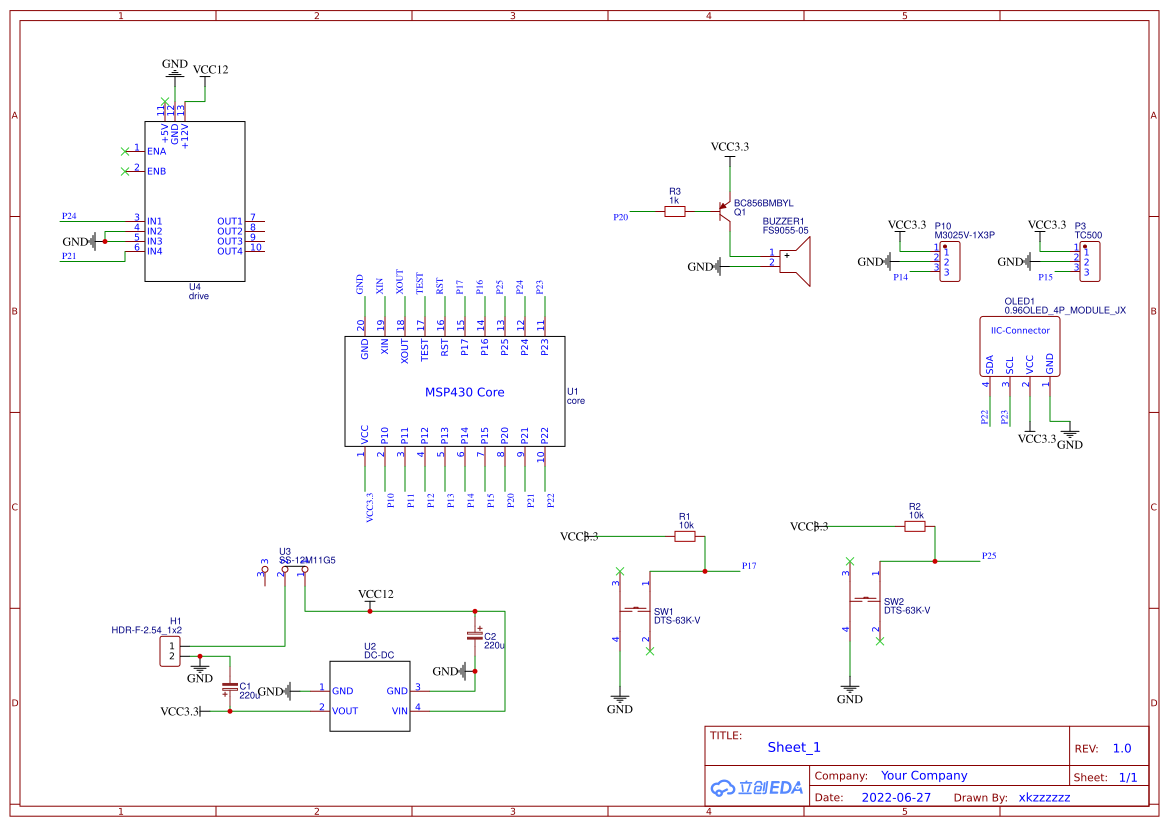
\includegraphics[width=0.5\textwidth]{Schematic.png}
\end{figure}

封装如图~\ref{fig:package},PCB的正反面如图~\ref{fig:pcb}。实物图如图~\ref{fig:real}。

\begin{figure}[htbp]
	\centering
	\caption{封装}
	\label{fig:package}
	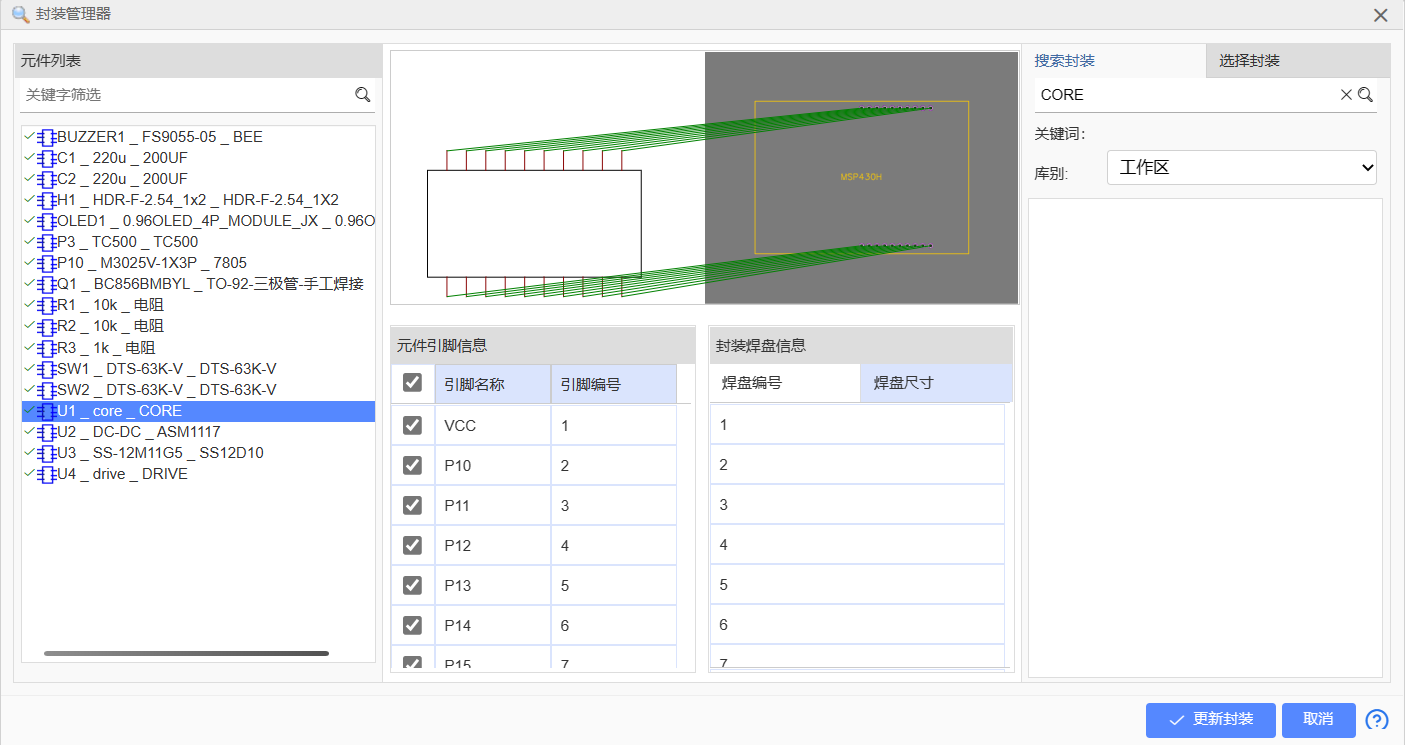
\includegraphics[width=0.6\textwidth]{package.png}
\end{figure}


\begin{figure}[htbp]
    \centering
	\caption{PCB}
	\label{fig:pcb}
	\subfigure[顶部]{
		\begin{minipage}[t]{0.48\linewidth}
			\centering
			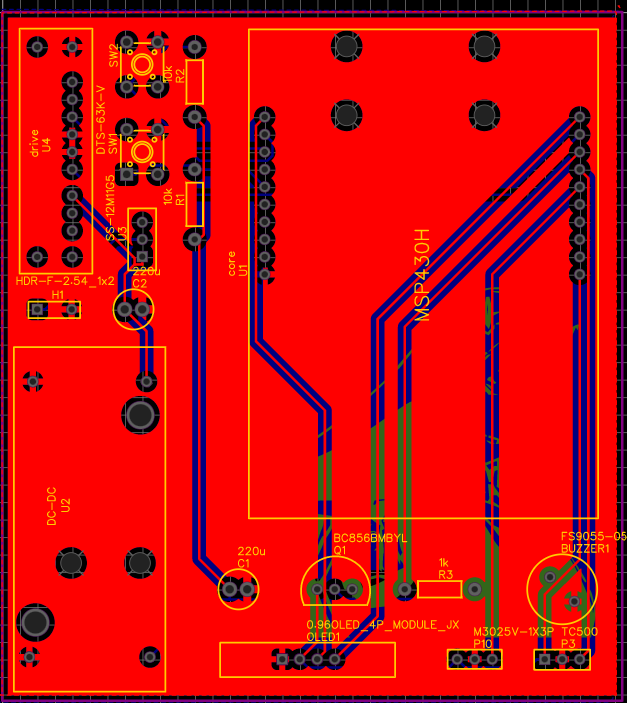
\includegraphics[width=0.8\textwidth]{pcb_top.png}
	\end{minipage}}
	\subfigure[底部]{
		\begin{minipage}[t]{0.48\linewidth}
			\centering
			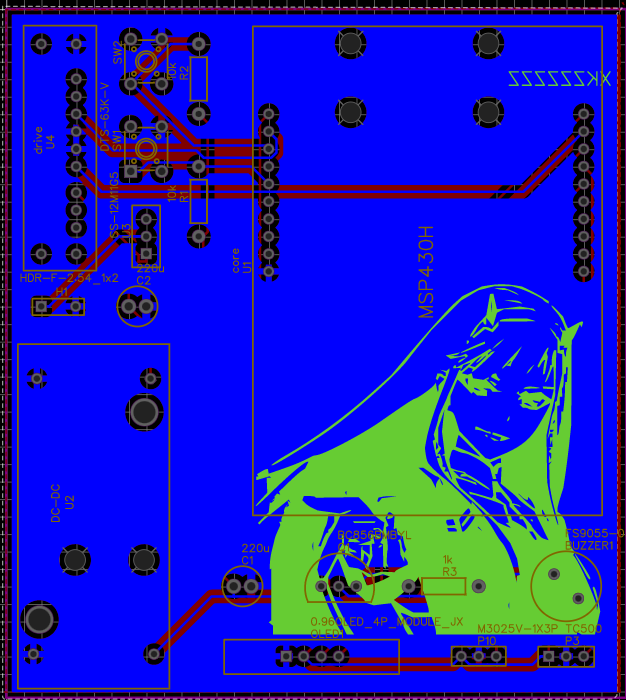
\includegraphics[width=0.8\textwidth]{pcb_bottom.png}
	\end{minipage}}
\end{figure}

\begin{figure}[htbp]
	\centering
	\caption{实物图}
	\label{fig:real}
	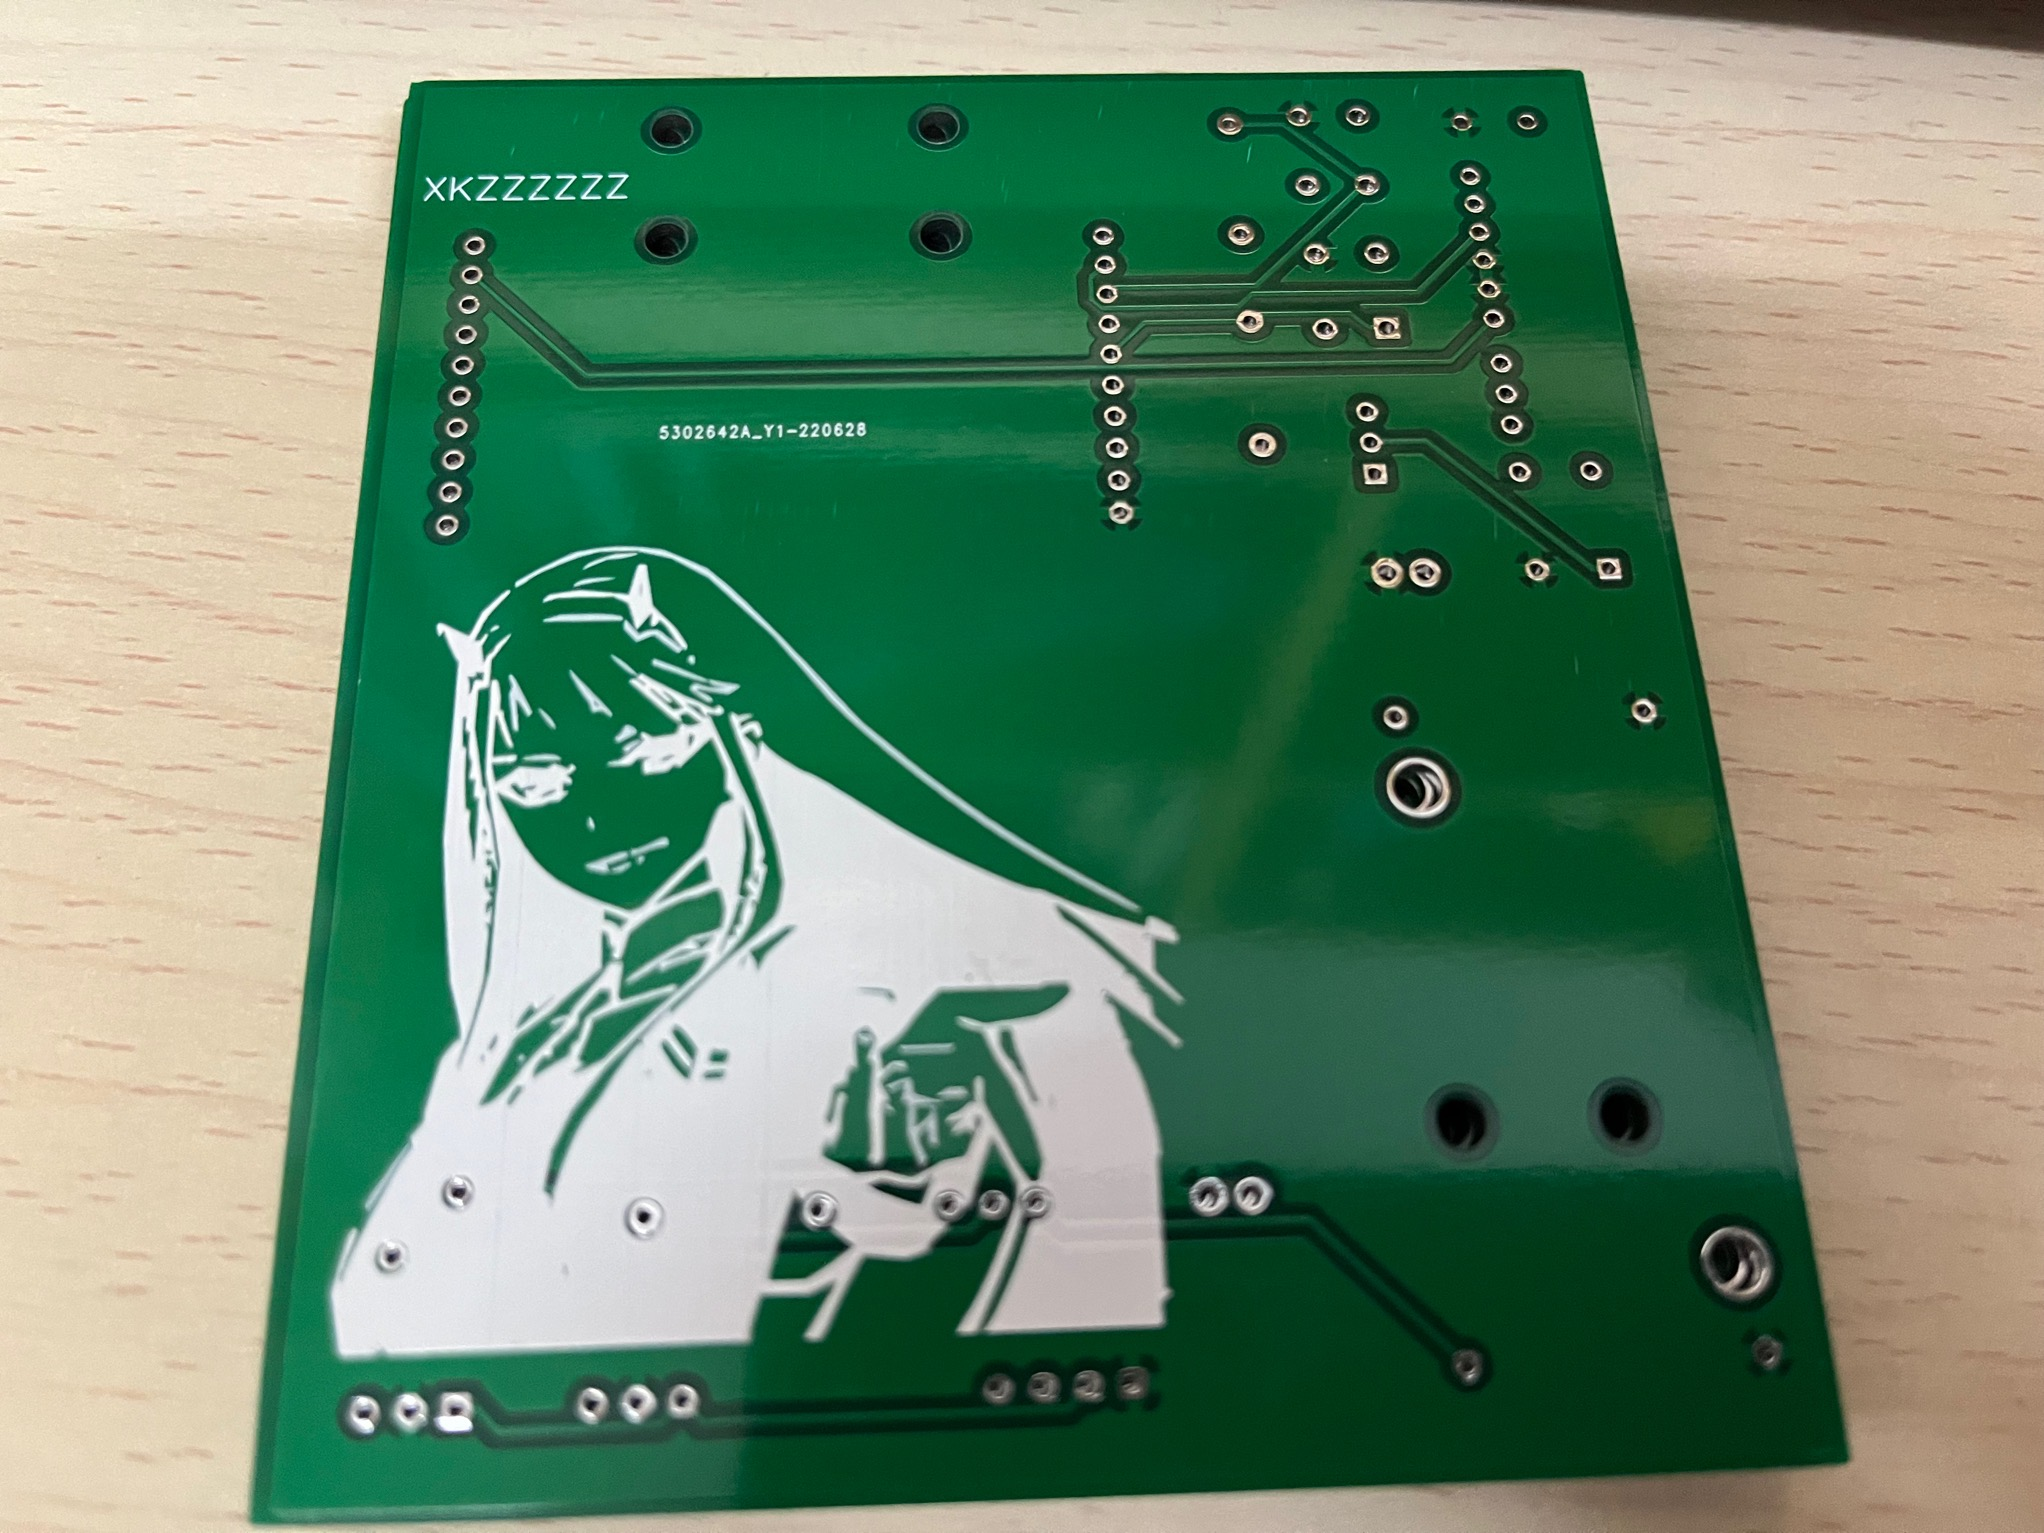
\includegraphics[width=0.6\textwidth]{real.jpg}
\end{figure}


\clearpage
\subsection{注意事项}

\begin{enumerate}
	\item 需要插接导线或者其它线缆的接口元器件一般放到电路板的外侧,
	并且接线的一面要朝外。例如,P1主控板插针一般放到电路板的外侧,
	使单片机接上后多余的部分露在外侧,减少占用PCB板空间。

	\item 元器件就近原则。元器件就近放置,可以缩短PCB导线的距离,
	如果是去耦电容或者滤波电容,越靠近元器件,效果越好。
	例如,H5和SW1就近放置,可以缩短PCB导线距离。

	\item 整齐排列。一个IC芯片的辅助电容电阻电路,围绕此IC把电阻电容整齐的排列,
	可以更美观。例如,R6、R7和C10、C8整齐排列,使整个电路板美观。

	\item 在排列放置元件时,要考虑到实际安装的要求,避免把针脚画反导致需要用线搭接。
\end{enumerate}

\subsection{主要挑战}

\begin{itemize}
	\item 封装:元件封装需要耐心和细心,为了取得良好的效果,我首先在库中寻找符合规格的封装,对封装间隔和引脚对不上的元件,仔细一个个测量修改。
	\item 布局:许多元件需要额外留空间才能放置,如主控板插针需要布局在PCB板外侧,突出的地方可以留在外部减少空间,
	LCD屏幕的位置需要预留出左右两侧较多的空间防止元件与屏幕干涉。
\end{itemize}

\subsection{个人总结和经验感受}

通过两天半的PCB电路板训练,从PCB原理图、封装、原理图库、PCB库、PCB布局、布线、覆铜,通过立创平台提交文件和订单,收到PCB板并运用到小车上,我学习了电路板设计制作和使用的流程。
对PCB的经验总结,就是要仔细地对元器件进行封装和检查,在设计时考虑布局的合理性。立创平台是功能强大的SaaS平台,使用非常方便,既有丰富的元件库,而且操作简单便捷,无需额外安装。
这两天半学到的技能对日后参加比赛、制作电子器件有很大的帮助。

\section{MSP430单片机部分}

CCS作为一款IDE在2020年代的视角下看是不合格的。它没有良好的代码智能提示和重构功能,
也不能很好地支持源代码版本控制工具,因此我使用VSCode+PlatformIO这一新平台完成了代码的编写
这款插件通过配置相应的选项可以完美地兼容MSP430G2553平台。如图~\ref{fig:platformio}

\begin{figure}[htb]
    \centering
	\caption{PlatformIO}
	\label{fig:platformio}
	\subfigure[PlatformIO启动页]{
		\begin{minipage}[t]{0.48\linewidth}
			\centering
			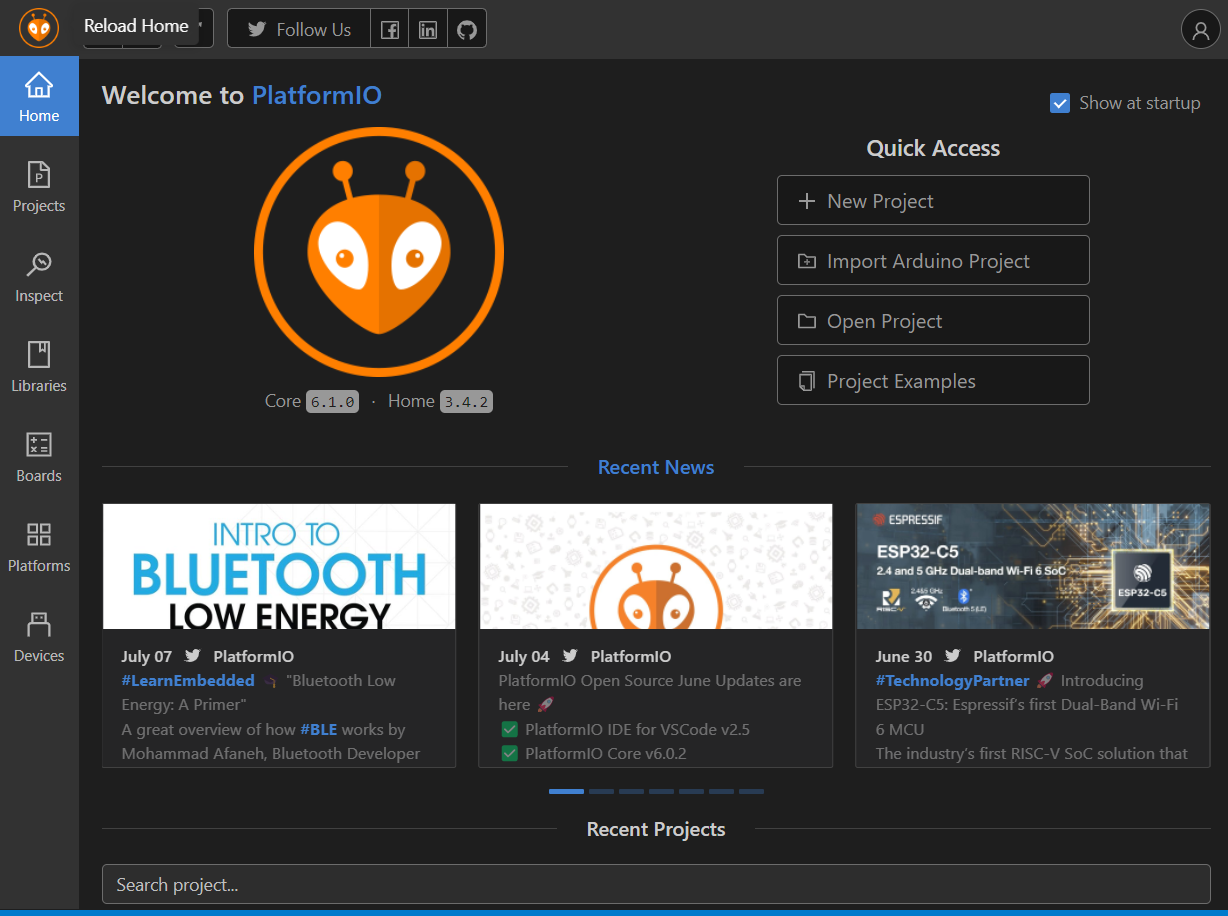
\includegraphics[width=0.8\textwidth]{platformio.png}
	\end{minipage}}
	\subfigure[相关配置文件]{
		\begin{minipage}[t]{0.48\linewidth}
			\centering
			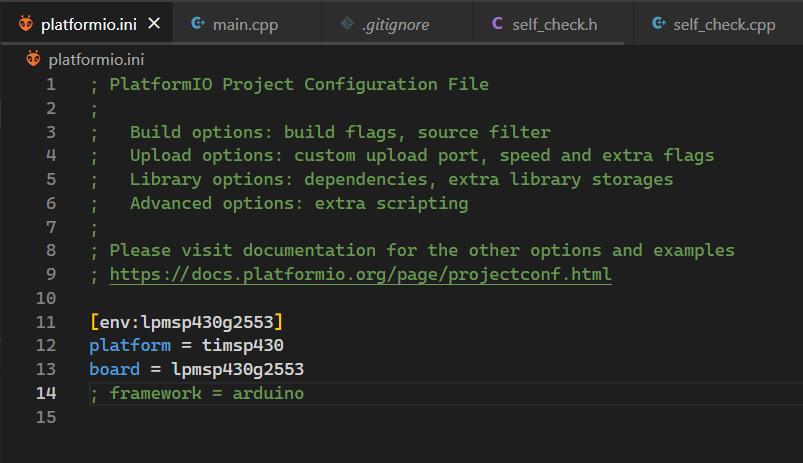
\includegraphics[width=0.8\textwidth]{platformio_cfg.png}
	\end{minipage}}
\end{figure}

\subsection{作业1}
读取 MSP430G2553 LaunchPad 上S2的按键状态,并用该按键控制LED1。按键按下时让LED 1亮起,按键松开时让LED 1熄灭。

\begin{lstlisting}[language=c++,numbers=left,style=CppStyle,caption=作业1,label={code:p1}]
#include <msp430.h> 
int main(void)
{
    WDTCTL = WDTPW | WDTHOLD;    // stop watchdog timer

    P1DIR |= BIT0;
    P1DIR &= ~BIT3;
    P1OUT|=BIT3;
    P1REN |= BIT3;

    while(1)
    {
        if(!(BIT3 & P1IN))
            P1OUT |= BIT0;
        else
            P1OUT &= ~BIT0;
    }
    return 0;
}
\end{lstlisting}

\subsubsection{现象和讨论}
MSP430G2553 LaunchPad 上 S2按键按下时让 LED 1亮起,按键松开时让 LED 1熄灭。
按键S2对应P1.3端口,设置P1.3为输入,LED1对应P1.0端口,设置P1.0为输出,使得按下S2时,
P1.0输出为0,让灯亮,松开时,P1.0输出为1,让灯灭。

在实现上,由于该程序比较简单,没有复杂的需求,对资源管理的要求不高,所以直接轮询而不是使用中断。
但这种方式可能浪费CPU资源,在更复杂的程序中应该使用中断。

\subsection{作业2}
在上一节Blink程序的基础上,将MCLK分别设置为1MHz和8MHz
并观察LED1闪烁的频率有何变化。

\begin{lstlisting}[language=c++,numbers=left,style=CppStyle,caption=作业2,label={code:p2}]

#include <msp430g2553.h>

void set_1mhz()
{
  BCSCTL1 = CALBC1_1MHZ; // Set range

  DCOCTL = CALDCO_1MHZ;

  BCSCTL2 &= ~(DIVS_3); // SMCLK = DCO = 1MHz
}

void set_8mhz()
{
  BCSCTL1 = CALBC1_8MHZ; // Set range

  DCOCTL = CALBC1_8MHZ;

  BCSCTL2 &= ~(DIVS_3); // SMCLK = DCO = 1MHz
}

int main()
{
  WDTCTL = WDTPW | WDTHOLD; // stop watchdog timer
  P1DIR |= 0x01;            // configure P1.0 as output

  set_1mhz();
  //set_8mhz();

  volatile unsigned int i; // volatile to prevent optimization

  while (1)
  {
    P1OUT ^= 0x01; // toggle P1.0
    for (i = 10000; i > 0; i--)
      __delay_cycles(10); // delay
  }
  return 0;
}
\end{lstlisting}

\subsubsection{现象和讨论}
通过对比将主时钟设为1MHz和8MHz的情况下,能明显发现到8MHz下LED1闪烁频率比1MHz快。
可见,主时钟频率越大、每个时钟周期的时间就越短,相对来说运行就越快,但功耗也越多。


\subsection{作业3}
通过GPIO中断的方式,用两个按键分别控制两盏不同的LED灯。每按下一次按键,相应的LED灯改变一次亮灭状态。
提示:板子上只有一个按键S2,可以用杜邦线一端连接在GND或者VCC,另外一端触碰下自己选择的IO口,模拟按键按下的状态。


\begin{lstlisting}[language=c++,numbers=left,style=CppStyle,caption=作业3,label={code:p3}]

#include <msp430.h> 
#if defined(__TI_COMPILER_VERSION__) || defined(__IAR_SYSTEMS_ICC__)
#pragma vector=PORT1_VECTOR
__interrupt void Port_1(void)
#elif defined(__GNUC__)
void __attribute__((interrupt(PORT1_VECTOR))) Port_1(void)
#else
#error Compiler not supported!
#endif
{
    if(!(P1IN & BIT4))
    {
        P1OUT ^= BIT0;
        P1IFG &= ~BIT4;
    }
    if(!(P1IN & BIT5))
    {
        P1OUT ^= BIT6;
        P1IFG &= ~BIT5;
    }

}

int main(void)
{
    WDTCTL = WDTPW + WDTHOLD;   // stop watchdog timer
    P1DIR |= BIT0;
    P1OUT &= ~BIT0;

    P1DIR |= BIT6;
    P1OUT &= ~BIT6;

    P1DIR &= ~BIT4;
    P1OUT != BIT4;
    P1REN |= BIT4;

    P1DIR &= ~BIT5;
    P1OUT != BIT5;
    P1REN |= BIT5;

    P1IES |= BIT4;
    P1IFG &= ~BIT4;
    P1IE |= BIT4;

    P1IES |= BIT5;
    P1IFG &= ~BIT5;
    P1IE |= BIT5;

    __bis_SR_register(GIE);
    return 0;
}
\end{lstlisting}

\subsubsection{现象和讨论}
将C1接到单片机的GND端,R1对应开关S1接单片机P1.4端口,R2对应开关S2接单片机P1.5端口用来触发中断。
当对应开关(第一列前两行)按下时,对应端口由输出高电平变为输出低电平,对应LED灯就会改变一次亮灭状态,

\subsection{作业4}
编程实现:利用定时器编写呼吸灯。所谓呼吸灯是指LED在一个周期内先逐渐变亮,再逐渐变暗。

\begin{lstlisting}[language=c++,numbers=left,style=CppStyle,caption=作业4,label={code:p4}]

#include <msp430g2553.h>

int IncDec_PWM = 1;

int main(void)
{

  /*** Watchdog timer and clock Set-Up ***/
  WDTCTL = WDTPW + WDTHOLD; // Stop watchdog timer
  DCOCTL = 0;               // Select lowest DCOx and MODx
  BCSCTL1 = CALBC1_1MHZ;    // Set range
  DCOCTL = CALDCO_1MHZ;     // Set DCO step + modulation

  P1DIR |= BIT6;
  P1SEL |= BIT6;

  /*** Timer0_A Set-Up ***/
  TA0CCR0 |= 1000;           // PWM period
  TA0CCR1 |= 1;              // TA0CCR1 PWM duty cycle
  TA0CCTL1 |= OUTMOD_7;      // TA0CCR1 output mode = reset/set
  TA0CTL |= TASSEL_2 + MC_1; // SMCLK, Up Mode (Counts to TA0CCR0)

  /*** Timer1_A Set-Up ***/
  TA1CCR0 |= 2000;           // Counter value
  TA1CCTL0 |= CCIE;          // Enable Timer1_A interrupts
  TA1CTL |= TASSEL_2 + MC_1; // SMCLK, Up Mode (Counts to TA1CCR0)

  _BIS_SR(LPM0_bits + GIE); // Enter Low power mode 0 with interrupts enabled

  return 0;
}

#pragma vector = TIMER1_A0_VECTOR // Timer1 A0 interrupt service routine
__interrupt void Timer1_A0(void)
{

  TA0CCR1 += IncDec_PWM * 2;
  if (TA0CCR1 > 998 || TA0CCR1 < 2)
    IncDec_PWM = -IncDec_PWM;
}
\end{lstlisting}

\subsubsection{现象和讨论}
通过实验现象可以发现LED在一个周期内先逐渐变亮再逐渐变暗。通过不断设置CCR1的值不断变大,
调节PWM占空比,使得LED灯逐渐变亮,然后当达到最亮后,通过设置CCR1的值不断减小,
,调节PWM占空比,使LED灯逐渐变暗。

\subsection{作业5}
编写接收程序和发送程序,当开发板串口接收到PC机发来的字符“1”时,点亮LED1,并向PC机发送“LED\_ON”;
当当开发板串口接收到PC机发来的字符“0”时,熄灭LED1,并向PC机发送“LED\_OFF”;当收到其它字符时,翻转LED1状态,
并向PC机发送“LED\_ON”或者“LED\_OFF”,表明LED1当前的状态。

\begin{lstlisting}[language=c++,numbers=left,style=CppStyle,caption=作业5,label={code:p5}]

#include <msp430g2553.h>
#include <stdint.h>
#include <stdbool.h>

void set_1mhz()
{
  BCSCTL1 = CALBC1_1MHZ; // Set range

  DCOCTL = CALDCO_1MHZ;
}

void uart_init()
{
  UCA0CTL1 |= UCSSEL_2;
  UCA0BR0 = 104;
  UCA0BR1 = 0;
  UCA0MCTL = UCBRS0;
  UCA0CTL1 &= ~UCSWRST;
  IE2 |= UCA0RXIE;
}

void uart_puts(char *c)
{
  while (*c)
  {
    while (!(IFG2 & UCA0TXIFG))
    {
      __nop();
    }
    UCA0TXBUF = *c++;
  }
}

void __attribute__((interrupt(USCIAB0RX_VECTOR))) uart_rx_isr()
{
  volatile int led_on = !!UCA0RXBUF;

  if (led_on)
  {
    P1OUT |= BIT0;
    uart_puts("LED ON\n");
  }
  else
  {
    P1OUT &= ~BIT0;
    uart_puts("LED OFF\n");
  }
}

int main()
{
  WDTCTL = WDTPW | WDTHOLD; // stop watchdog timer

  P1DIR |= BIT0; // configure P1.0 as output
  P1OUT &= ~BIT0;

  DCOCTL = 0;
  set_1mhz();

  P1SEL = BIT1 | BIT2;
  P1SEL2 = BIT1 | BIT2;

  uart_init();

  __bis_SR_register(LPM0_bits | GIE);
  return 0;
}
\end{lstlisting}

\subsubsection{现象和讨论}
打开串口助手,当开发板串口接收到PC机发来的字符“1”时, LED1亮,并向PC机发送“LED\_ON”;
当开发板串口接收到PC机发来的字符“0”时,熄灭LED1,并向PC机发送“LED\_OFF”;
当收到其它字符时,翻转LED1状态,并向PC机发送“LED\_ON”或者“LED\_OFF”,表明LED1当前的状态。
函数$uart\_puts$用来向PC机发送字符串,中断函数接受PC机发来的字符,
字符为0则灯灭,为1则灯亮。

\subsection{作业6}

按如下格式在OLED屏上显示自己的姓名、学号和系别信息。

\begin{lstlisting}[language=c++,numbers=left,style=CppStyle,caption=作业6,label={code:p6}]

#include "msp430g2553.h"
#include"I2C_OLED.H"
#include"zimo.h"

#define LEN(arr) (sizeof(arr)/sizeof(arr[0]))

int name_indexes[]={1,2,7,8,9};
int major_indexes[]={5,6,10,11,12,13,14};
int sid[]={2,2,9,2,0,2,0,2,2,0,4,6,2,2};

int main(void)
{
   system_clock();
   I2C_OLED_Init();
   while(1)
   {
	   OLED_All(0);
//	   delay_ms(500);


	   volatile int i=0,cnt=0;
	   for(i=0;i<LEN(name_indexes);i++)
	   {
	       OLED_P16x16Ch((cnt++)*16,0,name_indexes[i]);
	   }

	   i=cnt=0;
	   for(i=0;i<LEN(major_indexes);i++)
	   {
	       OLED_P16x16Ch((cnt++)*16,3,major_indexes[i]);
	   }

	   OLED_P16x16Ch(0,6,3);
	   OLED_P16x16Ch(16,6,4);
	   OLED_P6x8Str(32,6,"22920202204622");

	   for(;;);
   }
}
\end{lstlisting}

\subsubsection{现象和讨论}

通过字模软件,取出自己的姓名、系别、学号的字模,然后
填写到codetab.h文件中,同时在main.c函数中编辑显示的位置。
一个汉字的宽度是16,高度值是2。字母和数字的宽度则是8。
由于学号较长,所以使用较小的字体。


\section{基于MSP430的智能小车行驶}

\subsection{电路与程序设计}

\subsubsection{需求分析和设计思路}

\begin{figure}[htb]
	\centering
	\caption{总体设计流程图}
	\label{fig:flowchart}
	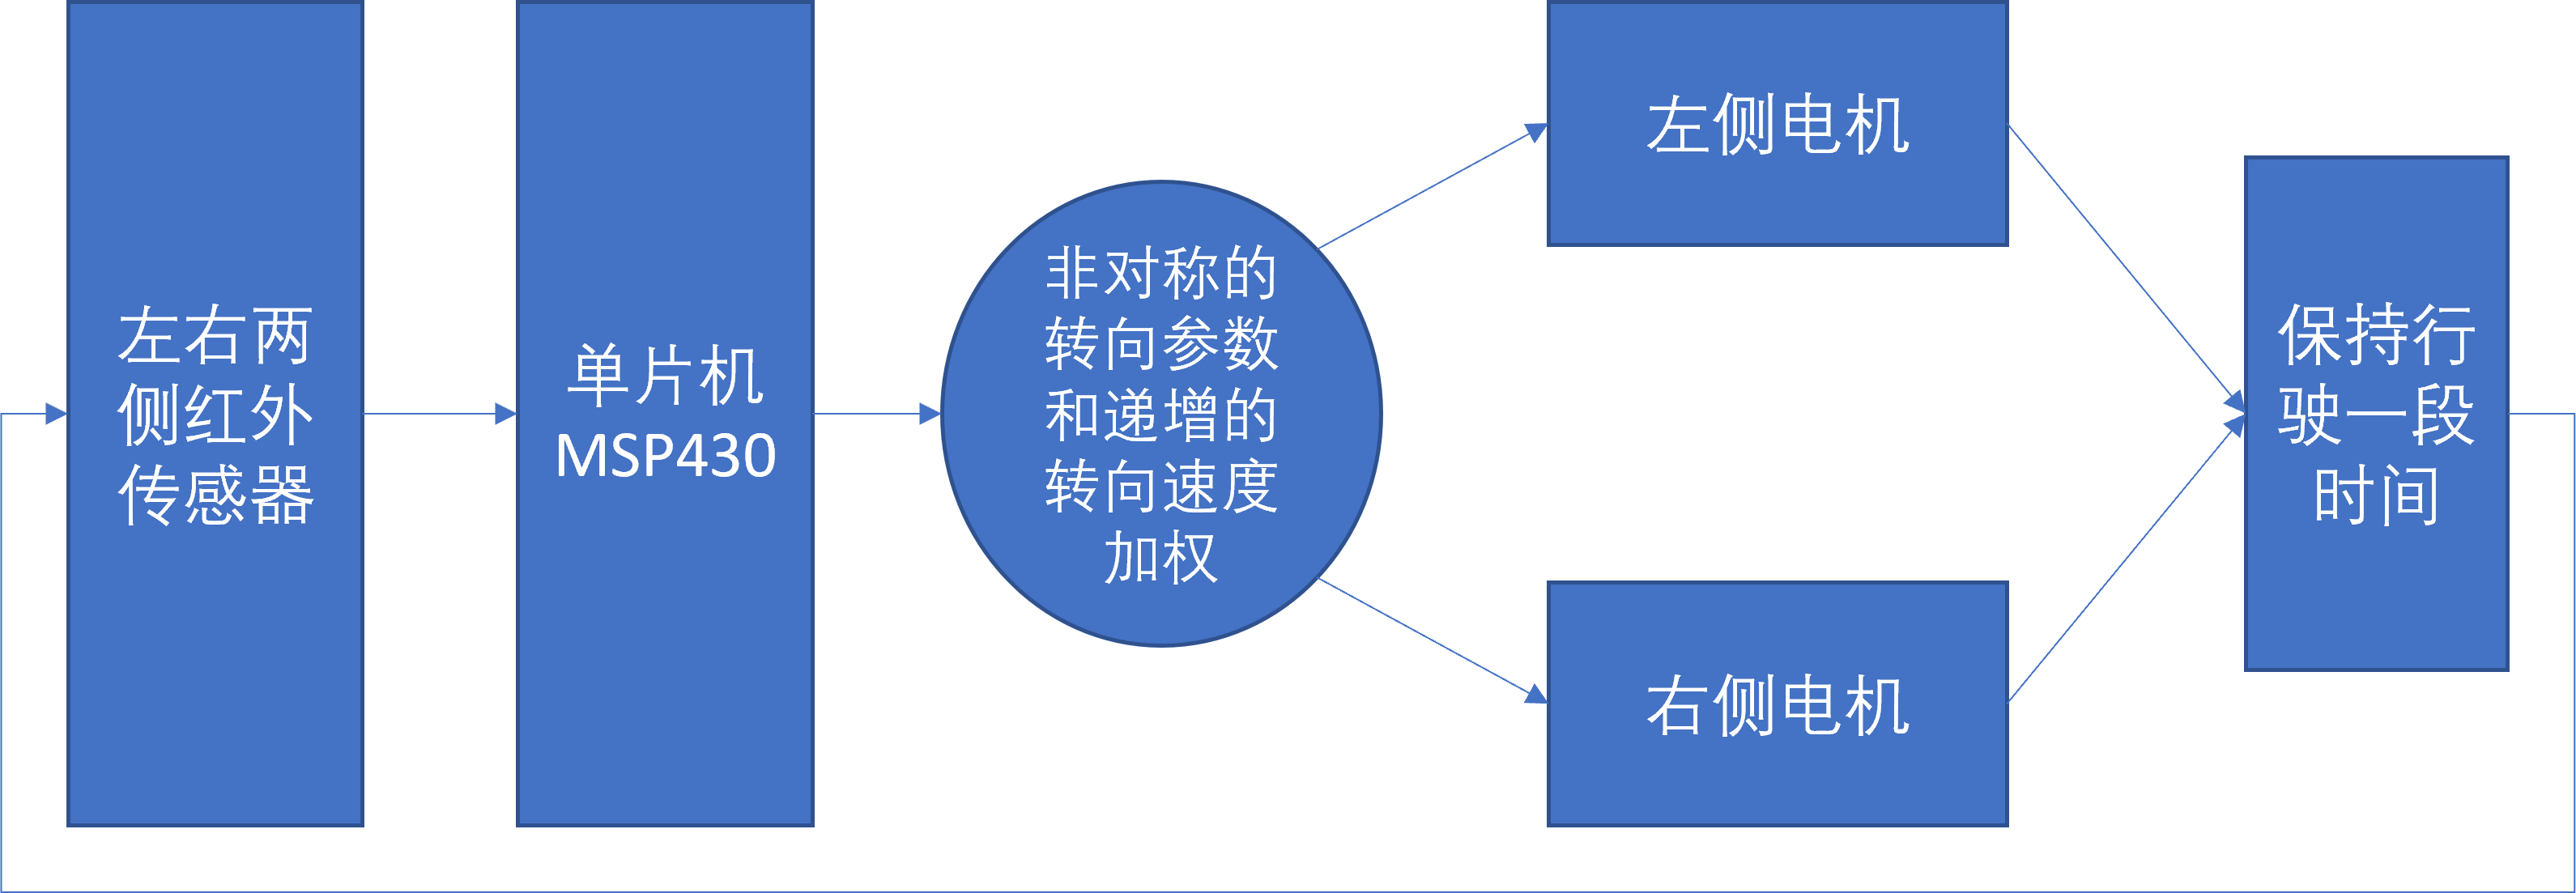
\includegraphics[width=0.9\textwidth]{flowchart.png}
\end{figure}

总体设计如图~\ref{fig:flowchart}。题目要求我们实现能够在地图上右转并停止的智能小车,时间可以在10s-20s之间调整。示意图如图~\ref{fig:car}(a)。
根据题目要求,我们需要实现转向功能。由于我们只有两个传感器,不能通过测量两次黑块的时间间隔获取速度信息,因此
我们退而求其次,将车轮可能的转速分为10档,通过试验测定挡位与用时的关系。

由于电机和轮子的设计存在公差、导线长度等原因,两侧速度不能完全一致,因此实际轨迹可能如图~\ref{fig:car}(b)
所示具有较多微调转弯和少量改变方向的转弯。由于红外传感器只能分辨黑色/非黑色,不能区分白色与木板底色,在改变
方向时由于两传感器都从白块穿过而跑出赛道的情况时有发生。因此需要设计更加稳定的、更加容错的转向方法。


\begin{figure}[htb]
    \centering
	\caption{小车赛道}
	\label{fig:car}
	\subfigure[赛道示意图]{
		\begin{minipage}[t]{0.48\linewidth}
			\centering
			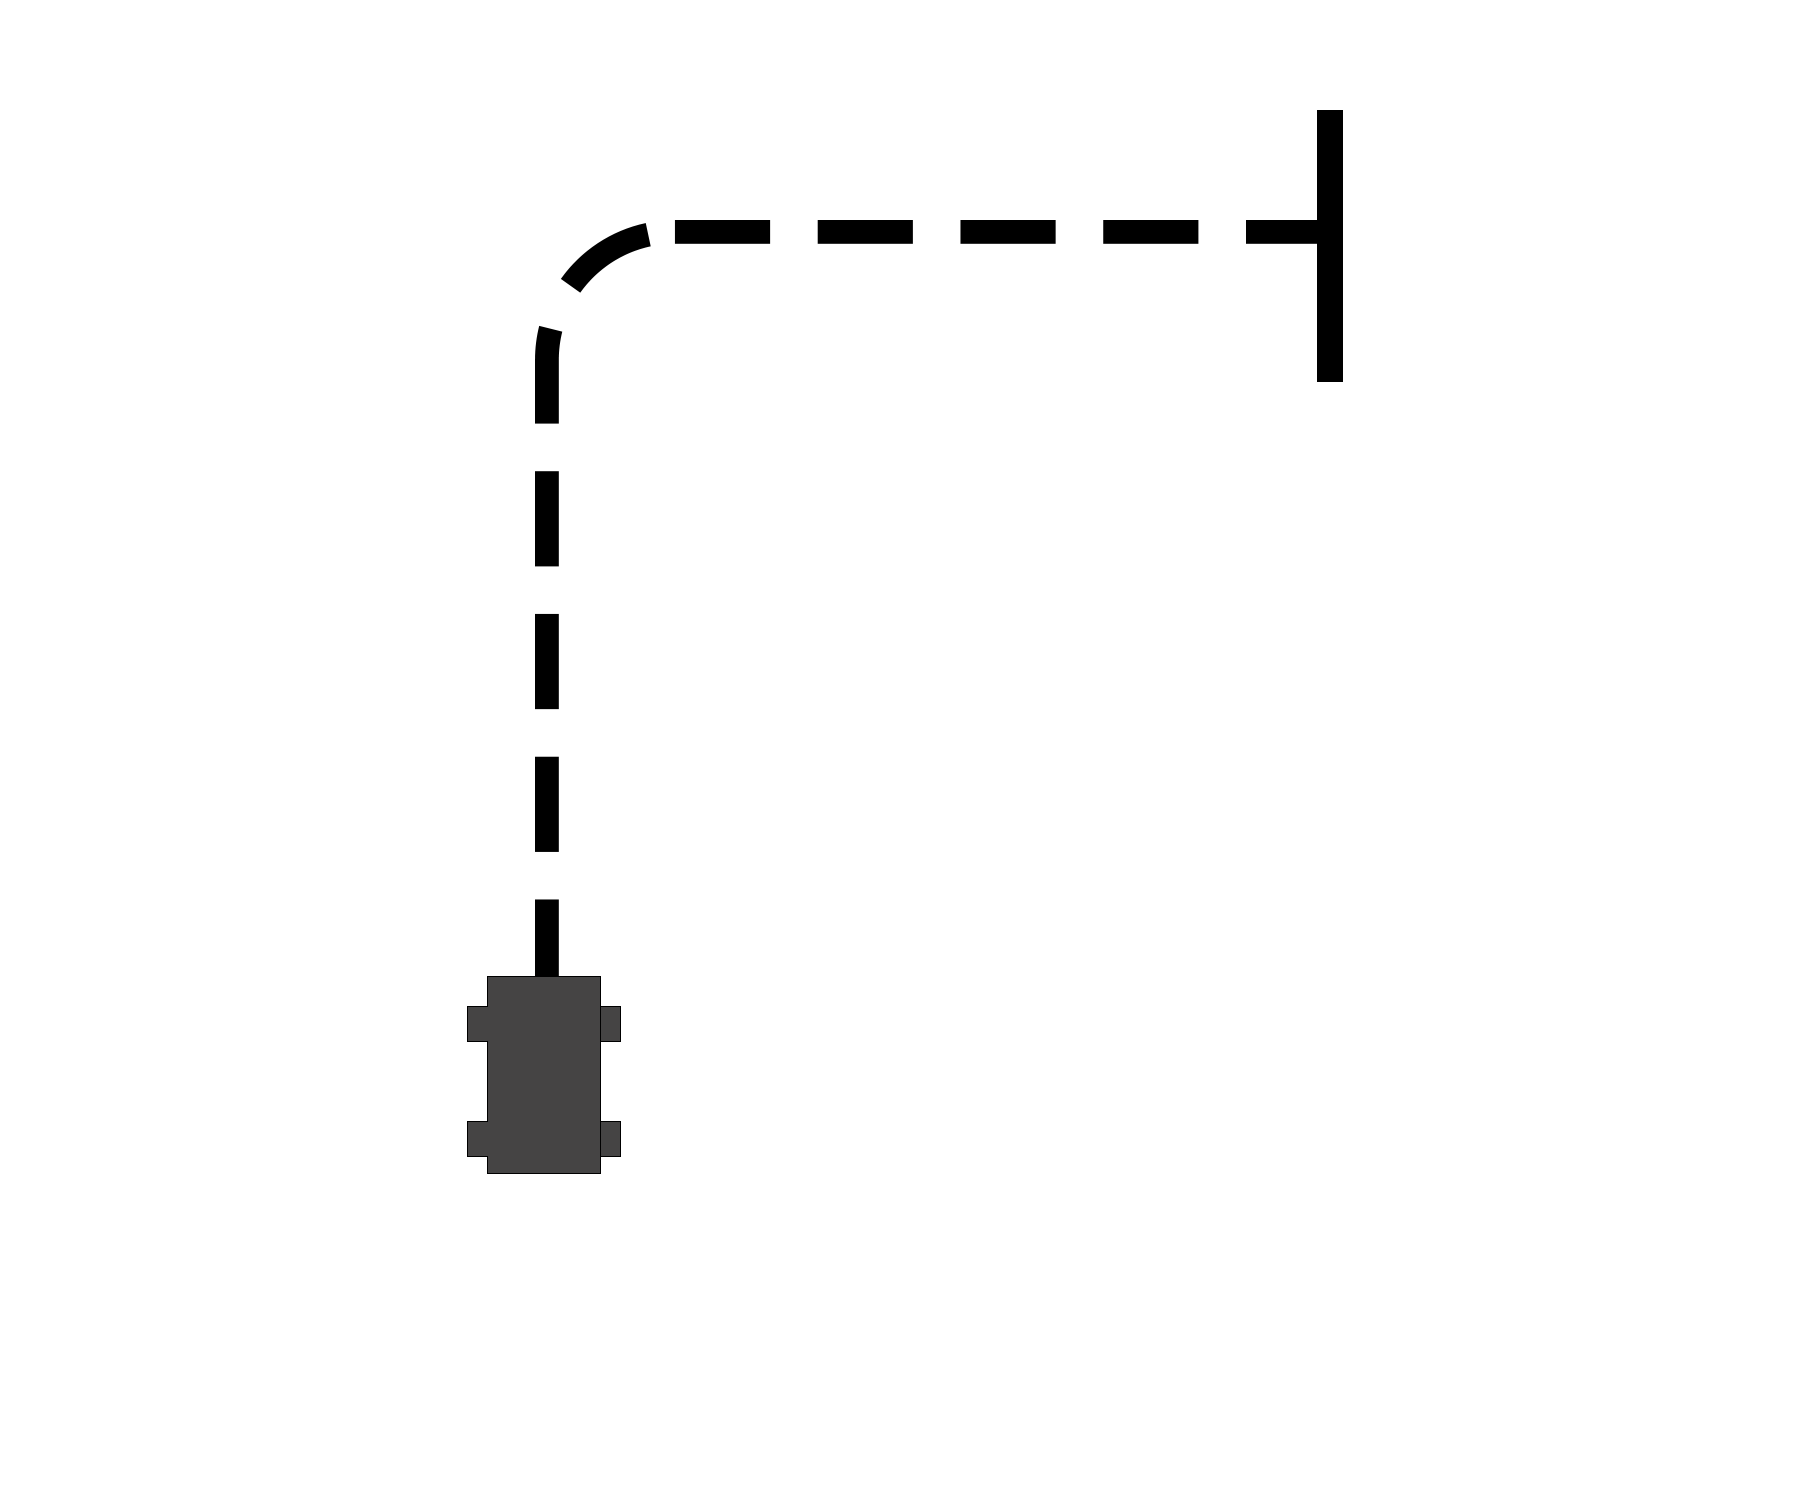
\includegraphics[width=0.8\textwidth]{car_track.png}
	\end{minipage}}
	\subfigure[轨迹示意图]{
		\begin{minipage}[t]{0.48\linewidth}
			\centering
			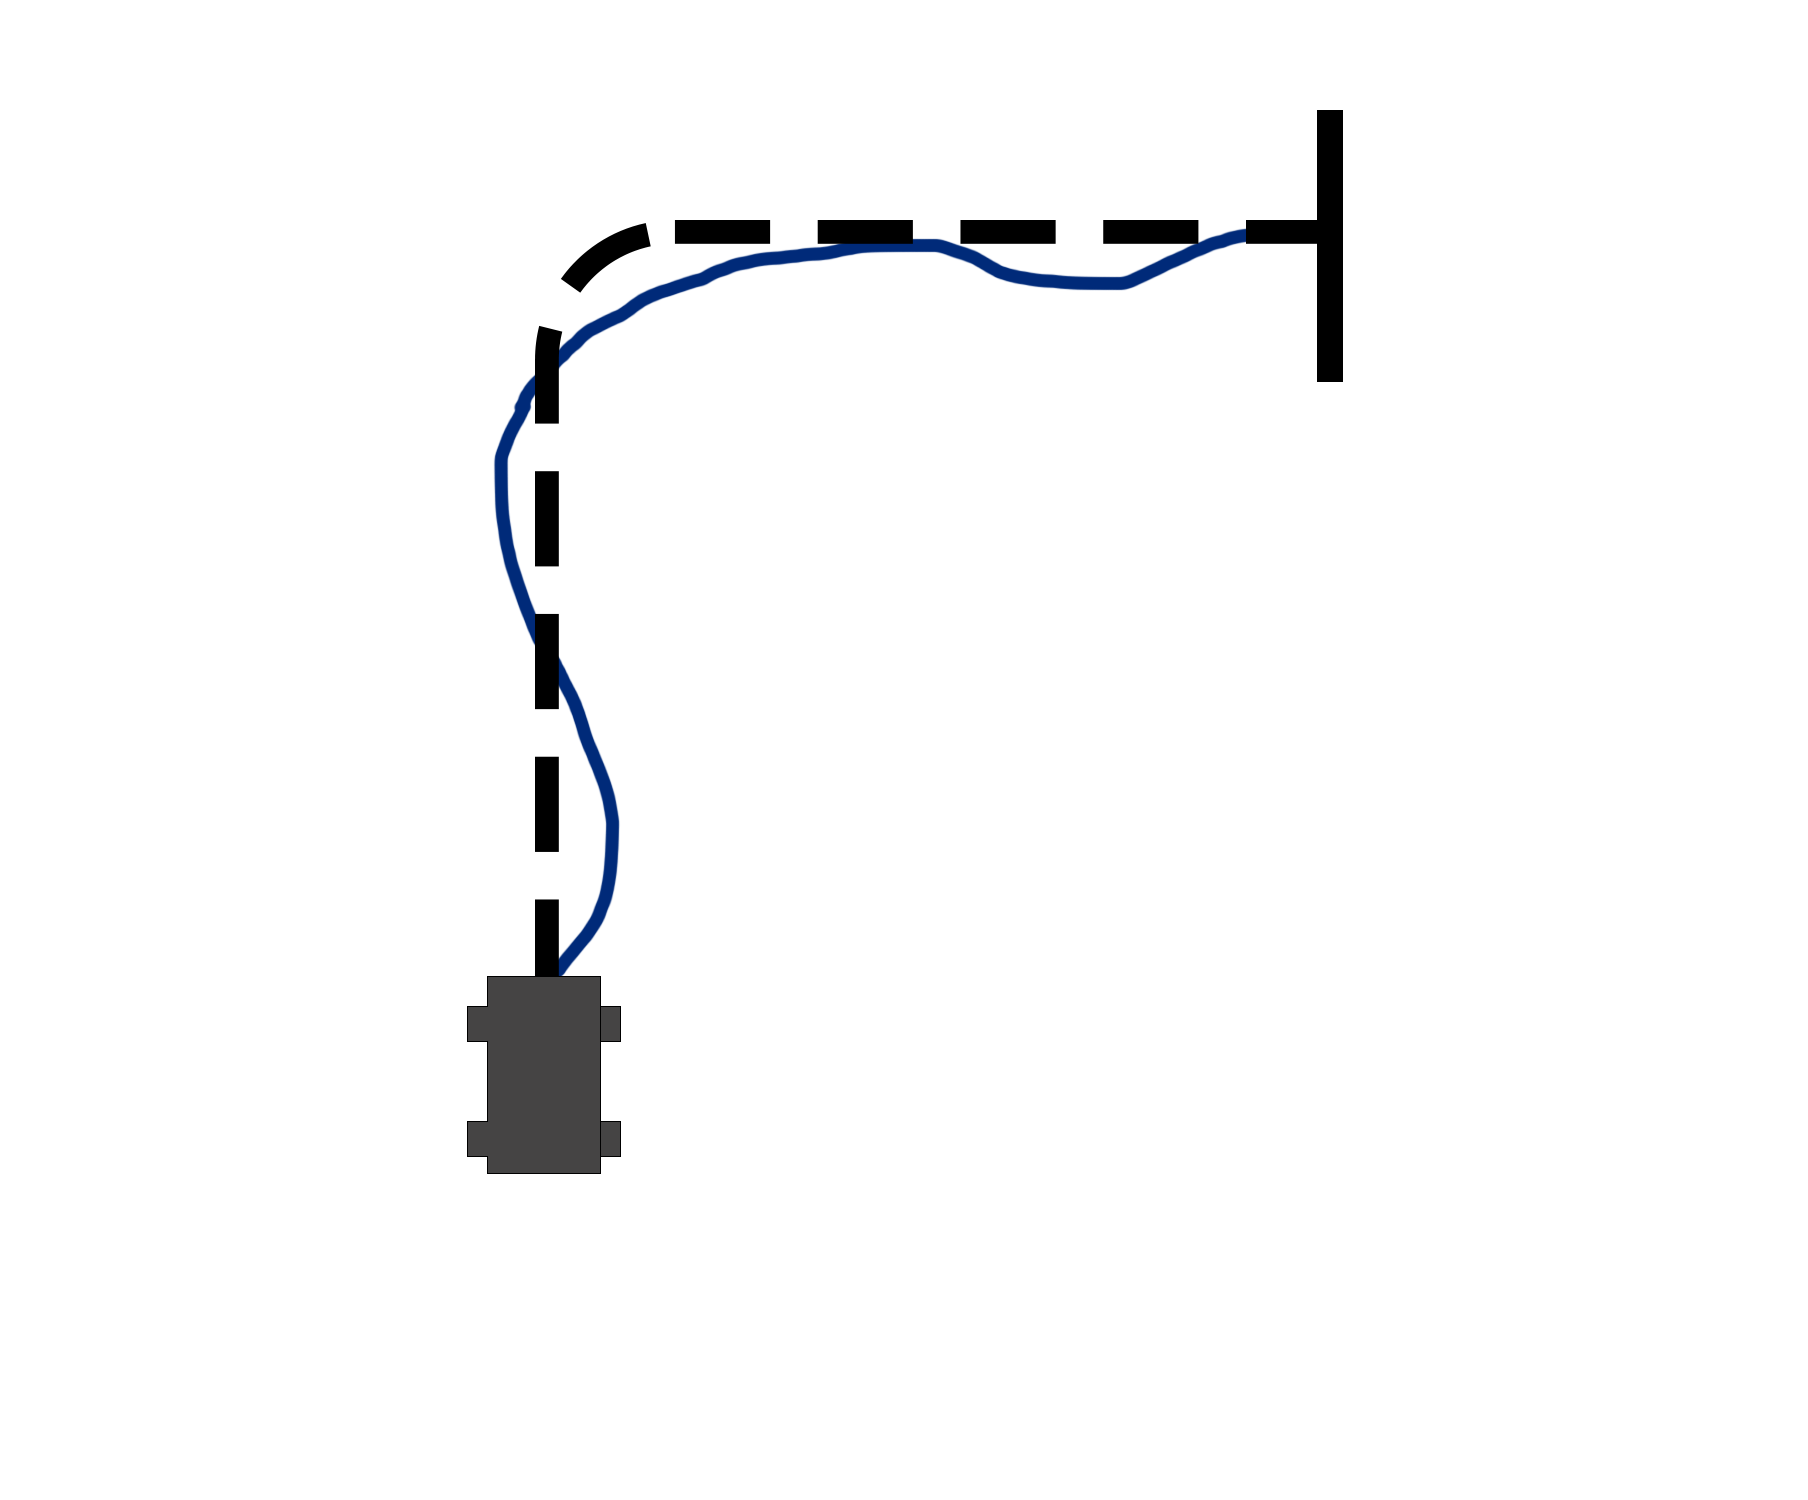
\includegraphics[width=0.8\textwidth]{car_track_example.png}
	\end{minipage}}
\end{figure}

\subsubsection{非对称的转向参数}

为了进行转向功能的具体实现,我们首先从需求出发进一步分析。由于赛道本身只向右转,因此所有的左转都是“微调转向”,
而右转包括“微调转向”和“变向转向”,这意味着左转的需求是微小的转向,而右转的转向则需要兼顾小转向和大转向的需要。

根据这一特征,我们可以对小车的控制加入归纳偏置来提高系统的稳定性。具体而言,我们对左转右转的控制采用了非对称的参数结构。
如表~\ref{tbl:turnparam}。

\begin{table}[htb]
	\centering
	\renewcommand\arraystretch{1.5}
	\caption{左转右转的参数}
	\label{tbl:turnparam}
	\begin{tabular}{c|c|c}
		\toprule
		\hline
		& 左转 & 右转 \\
		\hline
		参数类型 & 固定 & 可变 \\
		\hline
		转向轮速 & 左侧为右侧的80\%以上 & 右侧为左侧的2\%以下 \\
		\hline
		\bottomrule
	\end{tabular}
\end{table}

\subsubsection{递增的转向速度加权}

\begin{table}[htb]
	\centering
	\caption{加权函数}
	\label{tbl:weight}
	\renewcommand\arraystretch{1.5}
	\begin{tabular}{c|c}
		\toprule
		\hline
		权函数类型 & 表达式 \\
		\hline
		余弦型函数 & $y(k;n)=\cos(nk\pi)$ \\
		\hline
		多项式型函数 & $y(k;n)=a_nk^n+a_{n-1}k^{n-1}+\cdots+a_1k+a_0$ \\
		\hline
		指数型函数 & $y(k;a,m,n)=m\cdot a^k+n$ \\
		\hline
		\bottomrule
	\end{tabular}
\end{table}

为了适应转向大小的需求在行驶过程中的变化,我们对每一次转向进行动态的加权。我们设计了如表~\ref{tbl:weight}的加权函数
来对每一次转弯进行加权。根据我们对行驶过程的观察,我们选择了指数加权的方式,主要有以下原因:

\begin{figure}[htb]
	\centering
	\caption{函数图像}
	\label{fig:weight}
	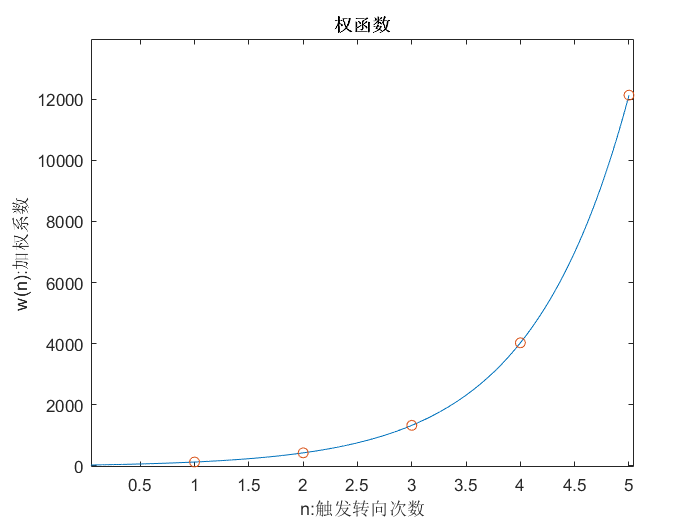
\includegraphics[width=0.48\textwidth]{weight.png}
\end{figure}

\begin{itemize}
\item 指数型函数的图像如图~\ref{fig:weight}。这符合转向需要逐步增大的需要。
\item 指数函数可以用如\eqref{eqn:recur_w}的形式递推地通过多项式实现,
可以减少进行复杂运算的需要。由于MSP430较弱的硬件性能,这能大大提高计算效率,
防止由于计算过于缓慢导致小车行驶不正常。
\end{itemize}

\begin{equation}
	\label{eqn:recur_w}
	y(k)=a\cdot y(k-1)+b
\end{equation}

经过这种加权处理,小车的转弯幅度依次增大,由于我们小车传感器右偏的设计,经过90°弯道
之后几乎不会触发转弯,因此可以达到稳定转向的目的。

同时,由于初期转向有
\begin{enumerate}
	\item 加权值较小
	\item 权函数增长缓慢
\end{enumerate}
的特点,小车在行驶初期较为稳定,避免了冲出赛道的事故发生。我们基于实践经验,将\eqref{eqn:recur_w}
中的参数设置为$a=3,b=40$,获得了较好的效果。

\subsubsection{方案合理性分析}
为了对选择一特定函数作为加权的方案能够产生很好的效果这一点给出合理的解释,
考察PID控制的公式\eqref{eqn:pid},
\begin{equation}
	\label{eqn:pid}
	u(n)=K_p\{e(n)+\frac{T}{T_I}\sum_{i=0}^ne(i)+\frac{T_D}{T}[e(n)-e(n-1)]\}+u_0
\end{equation}
该公式要求
\begin{enumerate}
	\item 对误差$e(n)$有一个较为准确的估计
	\item 积分项$\frac{T}{T_I}\sum_{i=0}^ne(i)$需要保存前$n+1$次的误差值
	\item 参数的计算涉及到浮点数的乘除
\end{enumerate}
很显然,由于只有两个红外传感器,要求1十分困难,甚至几乎不可能完美的实现;由于MSP430极为有限的性能约束,
要求2十分不现实,要求3很可能降低性能,然而积分控制是实现稳定的控制的必要要求,这产生了要求和能力之间的矛盾。

但是在现实环境中考量这一公式,对于一个长度不太长、变换不太大的赛道,转向的控制次数应当不太多,这意味着
转向控制量的值的变化大概率能够使用一个\emph{简单的}函数$w(n)$来进行\emph{相当精确的}近似。即\eqref{eqn:pid_approx}。
\begin{equation}
	\label{eqn:pid_approx}
	u(n)\approx K_p\cdot w(n)\cdot u_0
\end{equation}
这里的$w(n)$就是我们选择的加权函数。这个加权函数的效果就是同时近似比例项、积分项、微分项。依赖于\emph{转向次数不太多}这一假设,
这样的近似可以是非常精确的。

这种方案将能够解决上述提出的大多数困难。事实上,依赖于我们选择的指数型加权函数的递推形式,我们实现了移除所有的浮点数除法运算,将加法乘法
的计算量和对过往状态的存储量都降低到了常数级(\emph{与转向次数$n$无关}),这带来了可观的性能提升。

事实上,在只有两个传感器的情况下,我认为任何PID的实现都一定会引入一些(可能是隐式的)来自观察和试验的假设。而我们的工作将这中假设进行了
有效的形式化,大大提升了控制程序的可解释性,更加方便了选择、设计、分析与调试。虽然我们的方案在一定程度上牺牲了泛用性,引入了转向次数
不太多这一较强的假设,但是这种方案有相对完整的数学解释,并且在实际测试中有良好的表现。

\subsubsection{电路设计}

电路设计如图~\ref{fig:schematic2}。系统组成如表~\ref{tbl:system}

\begin{figure}[H]
	\centering
	\caption{原理图}
	\label{fig:schematic2}
	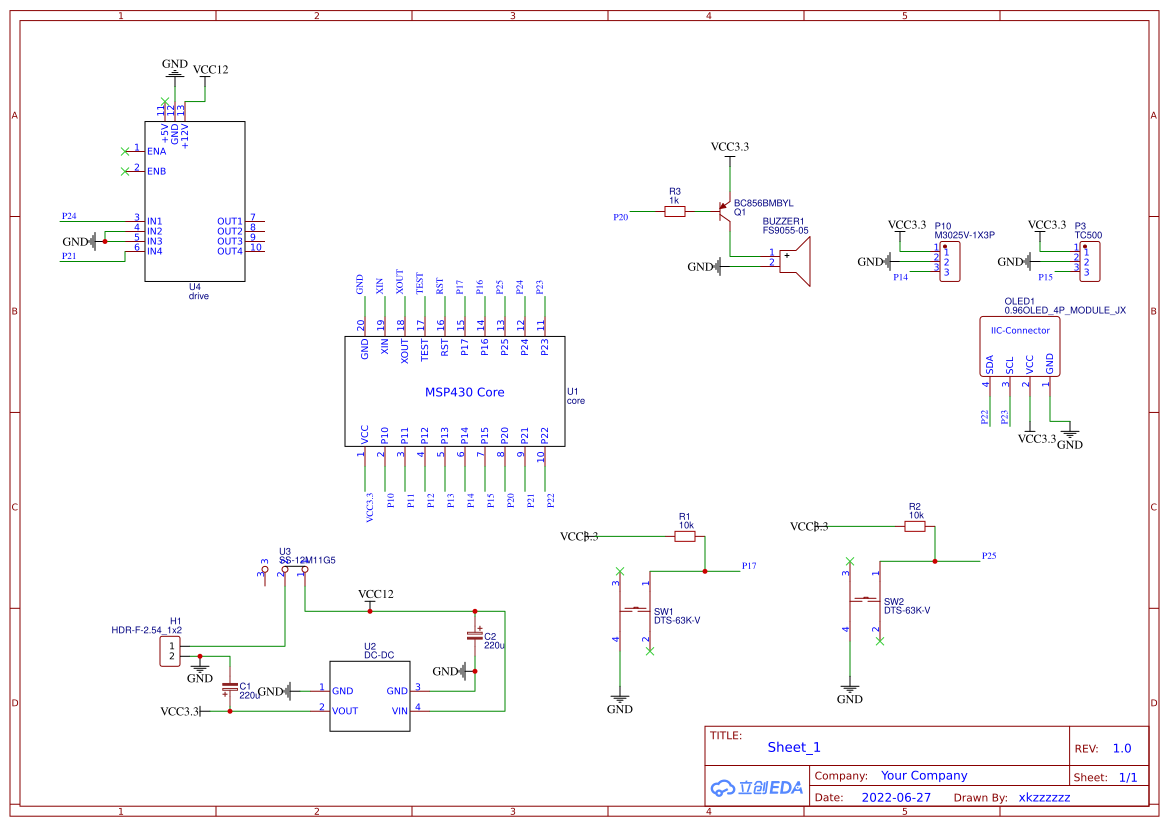
\includegraphics[width=0.6\textwidth]{Schematic.png}
\end{figure}

\begin{table}[H]
	\centering
	\renewcommand\arraystretch{1.5}
	\caption{系统组成}
	\label{tbl:system}
	\begin{tabular}{c|c}
		\toprule
		\hline
		显示模块 & OLED液晶显示 \\
		\hline
		供电方式 & 3节18650锂电池 \\
		\hline
		输入方式 & 红外循迹、按键 \\
		\hline
		输出方式 & 小车(2驱动+1万向轮)OLED显示屏 蜂鸣器 \\
		\hline
		控制芯片 & MSP430单片机(MSP430G2 launchpad) \\
		\hline
		制作工艺 & 印制电路板 \\
		\hline
		\bottomrule
	\end{tabular}
\end{table}


\subsection{测试方案与测试结果}

\begin{enumerate}
	\item \textbf{功能测试:}首先对小车的基本功能进行测试,一开始发现小车的电机运转方式奇怪而没有规律。但在按任何单片机外的
	按键的时候都会恢复正常。我们对小车的电路进行排查,由于按键会向单片机引脚输入低电平(接地),我们怀疑单片机接地不良引发了问题,
	因此进行测量,果然发现单片机接地处电位不正常,导致了单片机GPIO输出不正常。重新对GND对应的针脚进行焊接之后测量电位正常,
	测试小车工作正常。在测试场地调整红外传感器上的电位器后小车基本正常工作。

	\item \textbf{稳定测试:}为了测试小车运行的稳定性,我们调整初始放置的角度进行测试,发现小车都能正确调整方向回到轨道。
	因此小车在方向上有较好的稳定性。同时调整赛道坡道进行测试,发现坡道角较大的时候由于小车侧滑,传感器无法扫描到停止线
	因此无法正常停止。我们因此调整了传感器安装的位置,解决了这个问题。

	\item \textbf{挡位-时间测试:}为了控制速度,我们在设计程序时加入了10个速度级别,因此需要对速度级别对应的时间进行测量。
	进行计时之后得到了表~\ref{tbl:time}。
	\begin{table}[H]
		\centering
		\renewcommand\arraystretch{1.5}
		\caption{时间测量}
		\label{tbl:time}
		\begin{tabular}{c|c}
			\toprule
			\hline
			挡位 & 时间 \\
			\hline
			10 & 20s \\
			12 & 17s \\
			14 & 15s \\
			16 & 12s \\
			18 & 10s \\
			\hline
			\bottomrule
		\end{tabular}
	\end{table}
	根据测量结果,我们能灵活调节小车的行驶时间。
\end{enumerate}

\subsection{本人所做的工作}

在小车项目中我完成了程序的设计、测试和参数的调整。

\subsection{经验总结}

\begin{enumerate}
	\item 设计PCB板要考虑到安装的合理性。由于设计的有些紧密,我们安装LED屏幕时需要使用线接出来,
	造成了一定的不便。

	\item 在安装元件时要注意元件之间的相互关系。我们在焊接供电插口的时候由于没有注意插口朝向,与其他元件
	产生了干涉,不得不拆下来,由于残留焊锡堵住焊孔清理十分麻烦而处理了很长时间。

	\item 在进行调整的时候要做到统筹兼顾。在调试时不能只对代码进行修改,也要前瞻性地设计能够方便利用按钮等调整的参数,
	以及通过微调小车的结构设计、传感器的间距、位置等根据需求进行恰当的统筹安排。
\end{enumerate}

\subsection{个人感受}

通过这次制作小车的课题,我们在一个多星期的实训里收获颇丰。

一是对电子工艺设计中的理论和实际应用有了新理解。在实训过程中,我们需要对电路进行恰当的连接与设计,进而形成完整的小车结构,最后进行单片机的编程。
这一系列方法既要求全面的思考,也要求细致的实现,更要求对相关知识的理解与掌握。通过这一过程,我们不仅练习了嵌入式编程,更掌握了一些电路板设计和控制论中的理论知识,
还对这些知识的实际应用有了更深刻的体会。

二是团队协作和分工的能力得到了新提升。从设计,到电路板的选择和小车的焊接,到对参数调节和改进的一步步尝试,
再到最后形成完整的通过验收的小车,团队协作和分工贯穿始终。从小车的设计到实际实现的代码编写、调整,都离不开分工和合作。
在实训中,我们很好地锻炼了团队协作和分工的能力,让我们能够在今后的学习与生活中更好地与他人实现合作和交流。

三是实际编写代码实现想法和设计的能力得到了新锻炼。正所谓“力行而后知之真”,
在我们确定了和其他组不一样的控制方式之后,必须通过编写代码将理论和设计的方案落到实处才能顺利完成实训的任务。
在这次实训中,我们使用PlatformIO这一新平台完成了代码的编写,这既涉及到对新环境的配置,
也涉及到对我们设计的方案的正确实现。通过这次实训,我们培养的这些能力对以后的学习、竞赛乃至今后的工作都有着重要的意义。


\clearpage
\section{人工智能入门}

\subsection{一键完成商超商品识别模型部署}

\begin{figure}[H]
	\centering
	\caption{一键完成商超商品识别模型部署}
	\label{fig:ai1}
	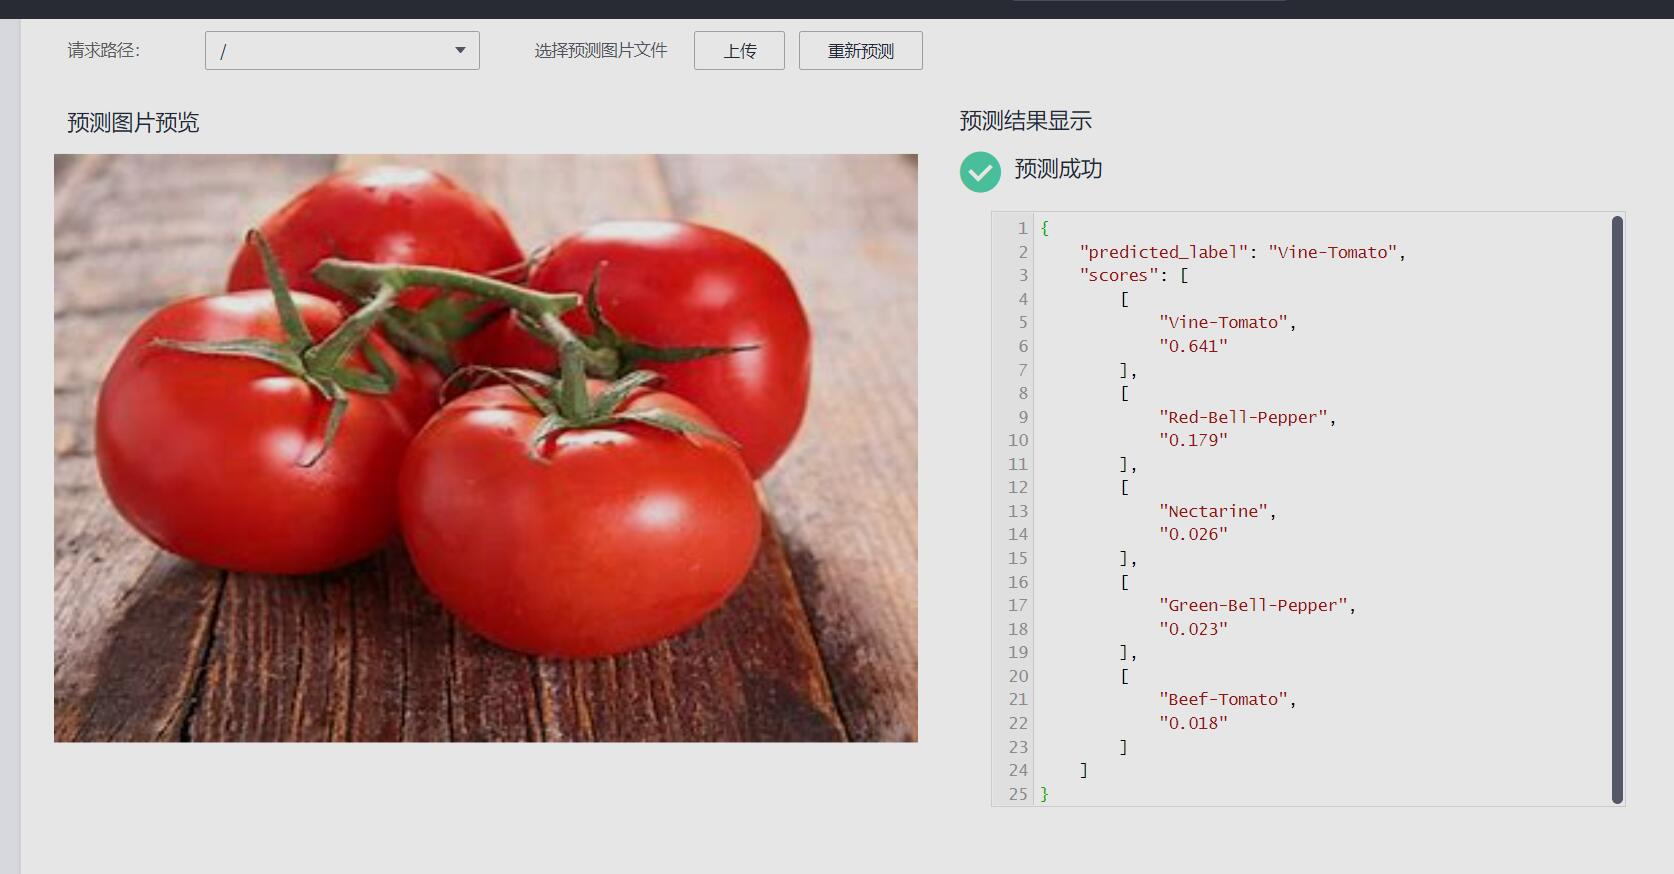
\includegraphics[width=0.68\textwidth]{task1.png}
\end{figure}

\subsection{一键运行 Notebook 实现工地钢筋盘点}

\begin{figure}[H]
	\centering
	\caption{一键运行 Notebook 实现工地钢筋盘点}
	\label{fig:ai21}
	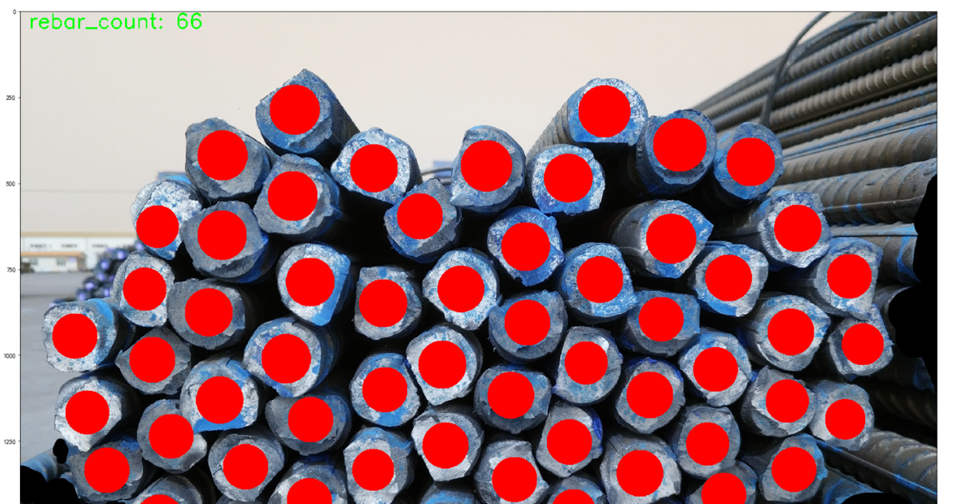
\includegraphics[width=0.8\textwidth]{task2_1.png}
\end{figure}

\begin{figure}[H]
	\centering
	\caption{一键运行 Notebook 实现工地钢筋盘点}
	\label{fig:ai22}
	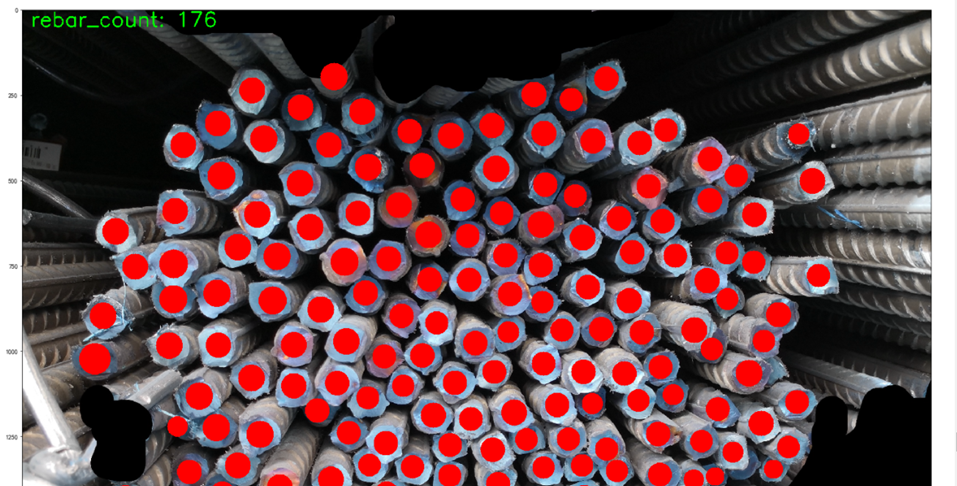
\includegraphics[width=0.8\textwidth]{task2_2.png}
\end{figure}

\subsection{使用自动学习0代码开发图像分类AI模型}

\begin{figure}[H]
	\centering
	\caption{使用自动学习0代码开发图像分类AI模型}
	\label{fig:ai31}
	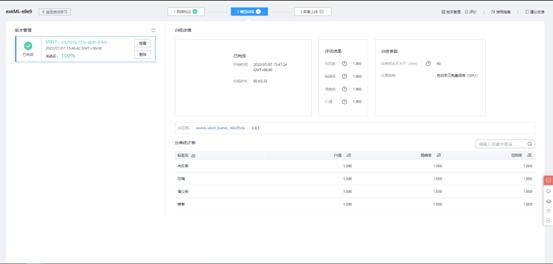
\includegraphics[width=0.8\textwidth]{task3_1.png}
\end{figure}

\begin{figure}[H]
	\centering
	\caption{使用自动学习0代码开发图像分类AI模型}
	\label{fig:ai32}
	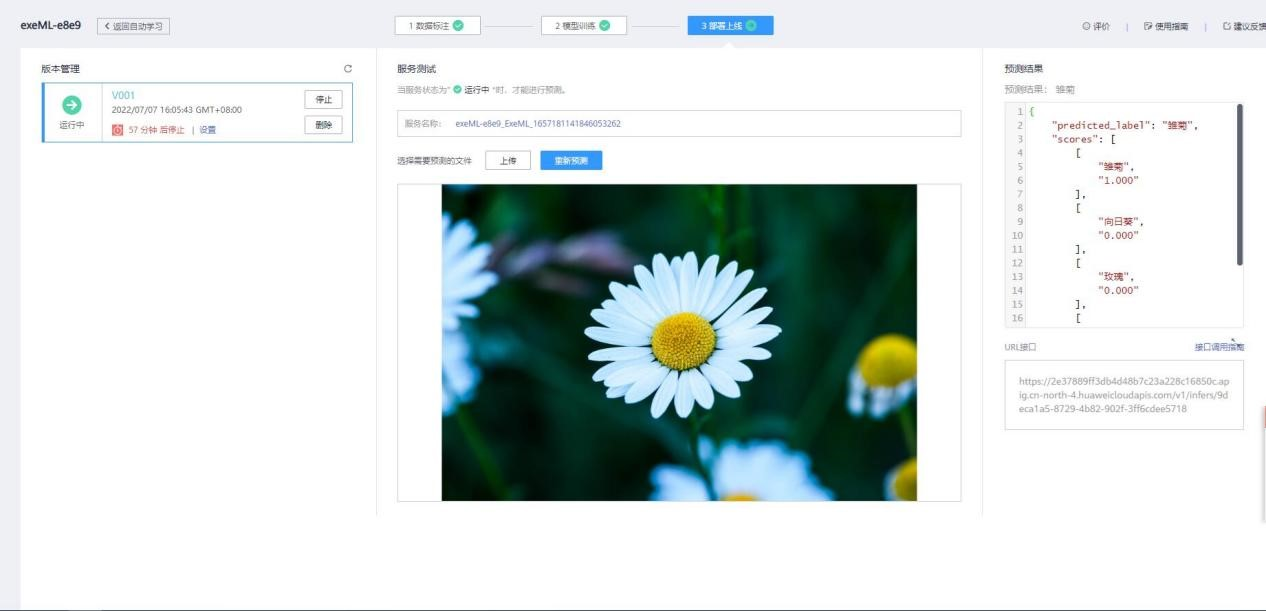
\includegraphics[width=0.8\textwidth]{task3_2.jpg}
\end{figure}

\subsection{使用订阅算法构建模型实现花卉识别}

\begin{figure}[H]
	\centering
	\caption{使用订阅算法构建模型实现花卉识别}
	\label{fig:ai41}
	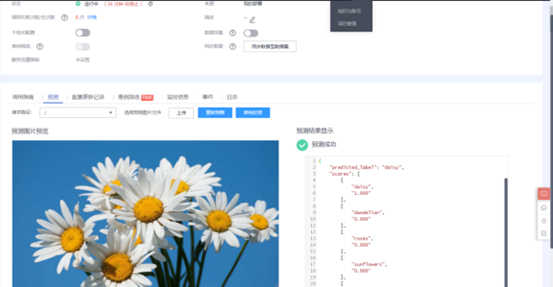
\includegraphics[width=0.8\textwidth]{task4.png}
\end{figure}

\subsection{使用时序预测算法实现访问流量预测}

\begin{figure}[H]
	\centering
	\caption{使用时序预测算法实现访问流量预测}
	\label{fig:ai51}
	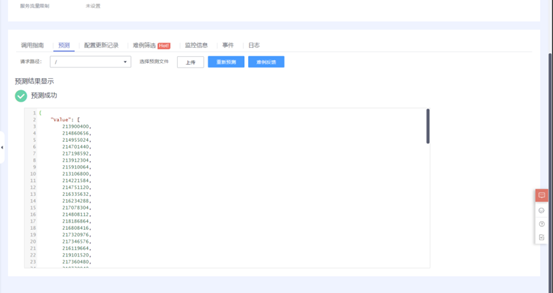
\includegraphics[width=0.8\textwidth]{task5.png}
\end{figure}

\subsection{在本地 PC 或者 ModelArts 里实现基于 MindSpore 的 MNIST 手写识别}

\begin{figure}[H]
	\centering
	\caption{测试图片}
	\label{fig:ai61}
	
\includegraphics[width=0.2\textwidth]{task6_1.jpg}
\end{figure}
\begin{figure}[H]
	\centering
	\caption{预测结果}
	\label{fig:ai62}
	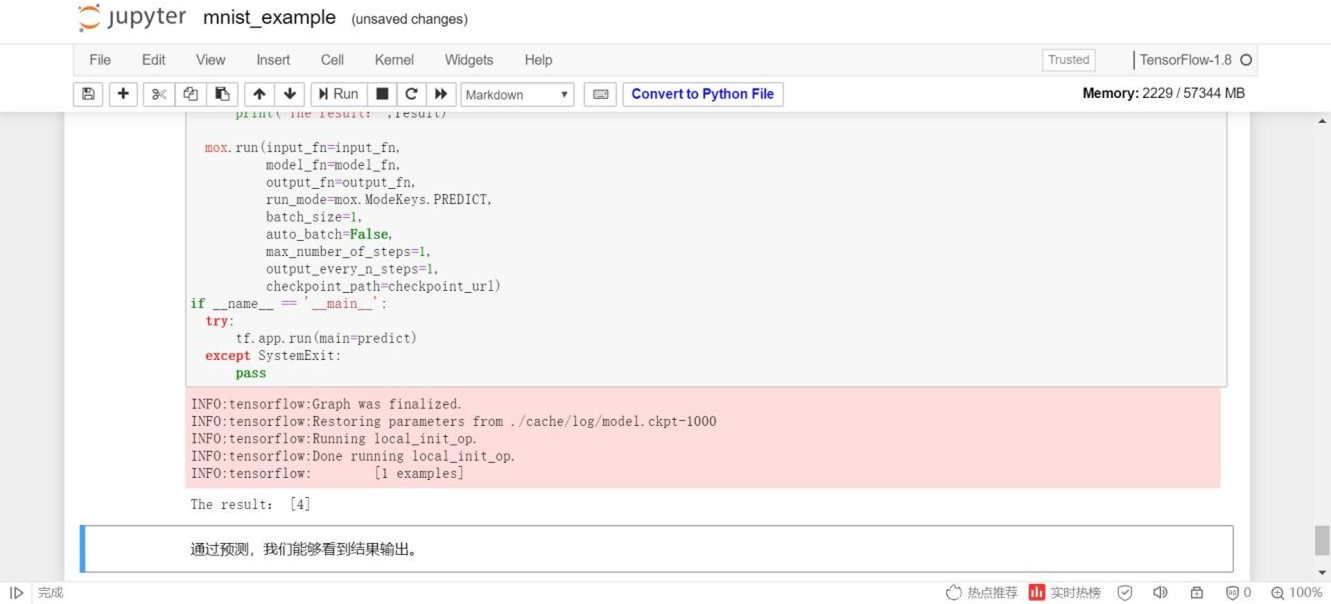
\includegraphics[width=0.8\textwidth]{task6_2.jpg}
\end{figure}

\clearpage
\section{实验改进建议}

\subsection{PCB制作}

PCB制作对计算机科学与技术的绝大多数同学来说都是第一次接触的、全新的一项技能。现在的课时安排有点紧、
对相关知识和操作的介绍比较简单,而且由于实验室桌子结构的原因坐在后排的同学对接受这些知识有更多的困难,
这导致了在布线、封装等比较精细考验技巧的环节大家都做的比较困难。

建议以后老师更详细地讲相关的知识,在实践过程中给更多的时间并多进行答疑,也可以从同学的结果中进行一定的检查
然后对问题进行集中的讲解。

\subsection{单片机编程}

在MSP430单片机学习过程中,老师把单片机时钟频率、中断、PWM等原理给我们讲述得很清晰,
但是硬件编程中对位运算等技巧的高度依赖对于大多数其他同学而言是很少接触的,因此对理解
实例代码产生了阻碍,希望老师在讲解这部分之前对相应的前置编程知识先进行一定的讲解。

此外,MSP430系列单片机较老、性能较弱、配套工具CCS使用体验较差。我在实践过程中使用VSCode和
PlatformIO的工具组合来解决了CCS使用体验差的问题,但单片机性能的问题既限制了程序的编写,
也不利于呈现硬件编程在当下的最佳实践,练习和发展趋势接轨的相关技能。希望换成STM32等较为强大的单片机
或者使用树莓派Zero这一小型化的开发板,如图~\ref{fig:rpi0},它不像普通的树莓派一样可以直接运行Linux操作系统,
因此也能用于练习嵌入式编程,并且它支持的MicroPython的编程上手也更加简单,适合在短短两周的实训过程中学习。

\begin{figure}[htb]
	\centering
	\caption{树莓派Zero}
	\label{fig:rpi0}
	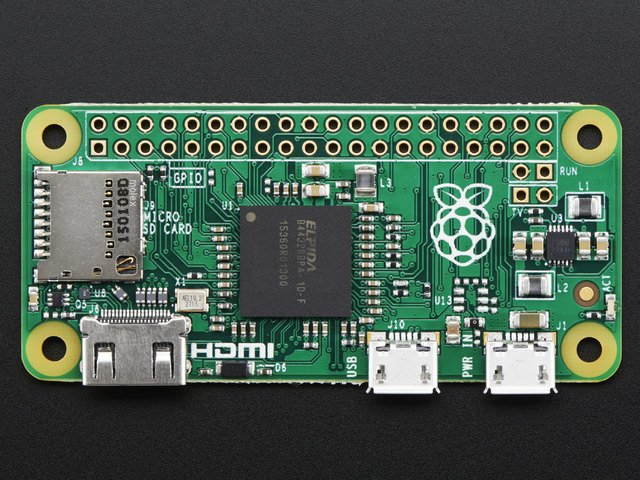
\includegraphics[width=0.48\textwidth]{rpi0.jpg}
\end{figure}

\subsection{MSP430小车}

小车制作是相对比较复杂、持续时间最长的一个模块。

首先,在电路板设计方面希望老师对各元件封装的参数和元件安装时的尺寸给更详细的文档,
来避免差错和安装时相互干涉导致的不便。

在安装调试小车前,如果能对吸锡器等外围工具的使用有一个简单的培训,就能更有效率地
上手相关工作。同时我们教室出现了小车冒烟起火的一起事故,在小车初次上电前应当请
同学仔细检查,防止锂电池可能出现的危险。

\subsection{人工智能}

人工智能部分的课时较少、实践时间较短、任务较重。我认为最好将人工智能和小车结合起来,
通过计算机视觉给小车导航既能锻炼制作小车时需要的电子设计技能,又能让我们对使用
人工智能解决实际问题有更好的体会。

\clearpage

\appendix
\section*{附录:小车控制行驶参数部分代码}

小车行驶参数控制(速度与转向)部分的代码如~\ref{code:carctl}

\begin{lstlisting}[language=c++,numbers=left,style=CppStyle,caption=作业6,label={code:carctl}]

#define TURN_DELAY 200

int turn_constant = 30;
const int turn_multipier = 3;
const int turn_bias = 40;
#define TURN_MAX 120

int delaytime;
void go()
{
  P2DIR |= (BIT1 + BIT4);
  P2SEL |= (BIT1 + BIT4);
  TA1CCR0 = 20000;        
  TA1CCTL1 = OUTMOD_7;
  TA1CCR1 = 0; 
  TA1CCTL2 = OUTMOD_7;
  TA1CCR2 = 0; 

 
  TA1CTL = (TASSEL1 + ID0 + ID1 + MC0);

  while (1)
  {
    OLED_ShowChar(80, 0, t_miao / 100 + '0'); 
    OLED_ShowChar(88, 0, t_miao % 100 / 10 + '0');
    OLED_ShowChar(96, 0, t_miao % 10 + '0');

    if (hy2 != 0 && hy1 != 0) 
    {
      TA1CCR1 = 0; 
      TA1CCR2 = 0;
      oled_puts(0, 0, "end ");

      while (1)
      {
        FM_L;
        delay_ms(100);
        FM_H; 
        delay_ms(100);
      }
    }
    else 
    {
      if (hy1 == 0) 
      {
        oled_puts(0, 2, "hy1 detect    ");
      }
      else
      {
        oled_puts(0, 2, "hy1 not detect");
      }

      if (hy2 == 0) 
      {
        oled_puts(0, 4, "hy2 detect     ");
      }
      else
      {
        oled_puts(0, 4, "hy2 not detect");
      }

      //  setmode=10-20  100-300 R
      if (hy1 == 0 && hy2 != 0) 
      {
        TA1CCR2 = (int)turn_constant * (100 + 20 * (setmode - 10)); 

        turn_constant = turn_multipier * turn_constant + turn_bias;
        if (turn_constant > TURN_MAX)
        {
          turn_constant = TURN_MAX;
        }

        if (setmode <= 13) 
        {
          TA1CCR1 = (int)10.5 * 30 * 0.2;
          delay_ms(TURN_DELAY);
        }
        else if (setmode <= 15)
        {
          TA1CCR1 = (int)10.5 * 50 * 0.2;
          delay_ms(TURN_DELAY);
        }
        else if (setmode <= 17)
        {
          TA1CCR1 = (int)10.5 * 60 * 0.2;
          delay_ms(TURN_DELAY);
        }
        else
        {
          TA1CCR1 = (int)10.5 * 70 * 0.2;
          delay_ms(TURN_DELAY);
        }
        delay_ms(30);
      }
      else if (hy2 == 0 && hy1 != 0)
      {
        volatile int speed = 30.5 * (100 + 20 * (setmode - 10));
        TA1CCR1 = (int)speed; 

        if (setmode <= 13)
        {
          TA1CCR2 = (int)speed;
          delay_ms(30);
        }
        else if (setmode <= 16)
        {
          TA1CCR2 = (int)speed * 0.8;
          delay_ms(30);
        }
        else
        {
          TA1CCR2 = (int)speed * 0.7;
          delay_ms(30);
        }
      }
      else if (hy1 == 0 && hy2 == 0)
      {
        TA1CCR1 = (int)30.5 * (100 + 20 * (setmode - 10));
        TA1CCR2 = (int)32 * (100 + 20 * (setmode - 10));
      }
    }
  }
}
\end{lstlisting}


\end{spacing}

\end{document}